\documentclass[10pt,letterpaper]{article}
\usepackage[utf8]{inputenc}
\usepackage{amsmath}
\usepackage{amsfonts}
\usepackage{amssymb}
\usepackage{gensymb}
\usepackage[margin=1in]{geometry}
\usepackage{graphicx}
\usepackage{hyperref}
\usepackage{subcaption}
\hypersetup{
    colorlinks,
    citecolor=black,
    filecolor=black,
    linkcolor=black,
    urlcolor=black
}
\begin{document}

\title{\scshape\LARGE University of Waterloo \vfill \bfseries PHYS 239 \\ \huge\bfseries Gravitational N-Body Problems\vfill }
\author{Jeremy Bullock, Robert Burnet, and Cliff Vong}
\maketitle

\newpage

\tableofcontents

\vfill

\section*{Individual Contributions}

Jeremy Bullock : Wrote the code for the simulation of Lagrange points of the Earth-Sun system.\\
Robert Burnet : Wrote code to test algorithms, as well as code for the simulation of galaxy collisions.\\
Cliff Vong : Wrote the code for the simulation of 3-body scattering.\\

\newpage


\section{Introduction}

We (Jeremy Bullock, Robert Burnet, and Cliff Vong) decided to study gravitational N-body problems. To study this, we needed a code that would calculate the trajectory of particles under the influence of gravity while conserving energy. We chose an ODE solver that conserved energy well, as well as calculated trajectories that agreed with known solutions, as failure to conserve energy will result in non-physical behaviour (such as orbits of 2-body systems growing in time). We investigate the Euler method, Euler-Cromer method, Midpoint method, Verlet method, and RK4 method to see which method gives the closest to expected results and conserves energy the best. The methods were tested by the following:\\

\begin{enumerate}
\item Simulated a projectile being thrown upward from the surface of the earth at varying velocities to test that the behaviour of the projectile agreed with the analytic solution.
\item Simulated the orbit of the moon around the earth to test for energy conservation, as well as to ensure we obtained the right orbital parameters (eg. orbital period of 27.373 days at position and velocity of Moon).
\end{enumerate}

The method that best agreed with the two above tests was found to be the RK4 method, so a decision was made to construct an N-body simulation of gravitating particles using the RK4 method of solving ODEs to calculate the particles' trajectories under gravity to study galaxy collisions, Lagrange points, and 3-body scattering.\\

For galaxy collisions, we simulated two massive bodies (one of $10^{11} M_\odot$ and another of $10^{10} M_\odot$) with massless particles positioned at random radial positions out to a radius of 30 kpc and 15 kpc respectively that are on a parabolic orbit (not head on) with respect to each other. The mass of the galaxies are concentrated at a point in which the massless particles that make up the rings of the galaxies orbit around. We produced images at specific times during the collision as well as an animations of the collision in this report and discussed what happens to the stars as well as the dependence of the collision on the angular momentum of orbiting stars relative to the angular momentum of the orbit (ie. prograde vs. retrograde orbits).\\

For Lagrange points, we studied specifically the Lagrange points of the Earth-Sun system. We introduced a massless third body placed at Lagrange points L2 and L4 and studied its orbit at each Lagrange point. We produced images of the orbit in the reference frame that is rotating with the Earth's orbit around the centre of mass of the system in this report and discussed whether or not these orbits are stable as well as what happens when we add a small change in the third body's momentum.\\

For 3-body scattering, we generated an initially stable binary star system and introduced a third massive body passing through the system and studied how it perturbs the system (ie. how it affects the energy of the system at late times) as well as whether or not its effect on the system depends on its initial velocity and position.\\
\newpage
\section{Algorithm Choices}
Here, we will discuss each of the methods in detail. We will refer the reader to the python code that is complementary to this report for the particulars of the code of the methods themselves.\\

The methods studied were the Euler method, Euler-Cromer method, the Midpoint method, the Verlet method and the RK4 method. These methods are compared against one another and their strengths and weaknesses are detailed. \\

\subsection{Euler Method}
The Euler method is a method of numerical integration that follows the following scheme:\\

\begin{equation}
\begin{split}
p_{n+1} & = p_n + h f(t_n, p_n)\\
\end{split}
\end{equation}\label{eqn:euler_method}

Where $p_n$ is the phase space coordinate of the system being integrated at the current time step, $h$ is a single step in time, and $f$ is a function which calculates the derivatives of the phase space coordinates at current time $t_n$ and current phase space coordinate $p_n$. This method is carried out until it reaches the final time step.\\

This method, while being computationally less expensive than the rest, fails to conserve energy as the derivatives are calculated strictly at the beginning of each time step, but are then applied to the whole time step, resulting in the solutions not being symmetric in time (ie. the same calculated forward as backwards). Thus, an integration method that is symmetric in time is better suited for conservating energy.\\

\subsection{Euler-Cromer Method}
The Euler-Cromer method arises from a modification of the Euler method that is more stable and time symmetric. It follows the following scheme:\\

\begin{equation}
\begin{split}
v_{n+1} & = v_n + a_n h\\
r_{n+1} & = r_n + v_{n+1} h\\
\end{split}
\end{equation}\label{eqn:euler_cromer_method}

Where $v_n$ and $r_n$ are the respective velocities and spatial coordinates of the system being integrated at the current time step, $h$ is a single step in time, and $a_n$ is the acceleration at the current time step. This method is known as a symplectic integrator as it conserves energy over the long-term. However, locally (ie. in small time ranges), there may be periodic fluctuations in the energy. A method which conserves energy without fluctuations would be preferable.\\

\subsection{Midpoint Method}
The Midpoint method is another modification of the Euler method that is more stable and time symmetric. It follows the following scheme:\\

\begin{equation}
\begin{split}
p_{n+1} & = p_n + h f(t_n + \frac{1}{2}h, p_n + \frac{1}{2} h f(t_n, p_n))\\
\end{split}
\end{equation}\label{eqn:midpoint_method}

Where $p_n$ is the phase space coordinate of the system being integrated at the current time step, $h$ is a single step in time, $f$ is a function which calculates the derivatives of the phase space coordinates at current time $t_n$ and current phase space coordinate $p_n$. This method gives the derivatives of the phase space coordinate evaluated between the current time step and the next time step, making it time symmetric. Like the Euler-Cromer method, this method is also a symplectic integrator as it conserves energy.\\

\subsection{Verlet Method}
The Verlet method is another method which is time symmetric and known as a symplectic integrator. It follows the following scheme:\\

First, initialize $r_1$.\\

\begin{equation}
\begin{split}
r_{1} & = r_0 + v_0 h + \frac{1}{2} a_0 h^2\\
\end{split}
\end{equation}\label{eqn:verlet_method_init}

Using the initial conditions of the phase space coordinates. Then for $n = 1, 2, ...$, iterate the following:\\


\begin{equation}
\begin{split}
r_{n+1} & = 2 r_n - r_{n-1} + a_n h^2\\
\end{split}
\end{equation}\label{eqn:verlet_method}
 
Where $r_n$ is the spatial coordinates at the current time step, $h$ is a single step in time, and $a_n$ is the acceleration at the current time step. This integration method is time symmetric and so is a viable candidate for energy conservation.\\


\subsection{RK4 Method} 
The fourth-order Runge Kutta (RK4) method is a higher order integration method than the above methods. It follows the following scheme:\\

\begin{equation}
\begin{split}
p_{n+1} &= p_n + \frac{1}{6}(k_1 + k_2 + k_3 + k_4)\\
k_1 & = h f(t_n, p_n)\\
k_2 & = h f(t_n + \frac{1}{2}h, p_n + \frac{1}{2}k_1)\\
k_3 & = h f(t_n + \frac{1}{2}h, p_n + \frac{1}{2}k_2)\\
k_4 & = h f(t_n + h, p_n + h k_3)\\
\end{split}
\end{equation}\label{eqn:rk4_method}

The Midpoint method is an example of a second-order Runge-Kutta method, so it is expected that RK4 should produce more precise results. However, generally speaking, Runge-Kutta methods do not conserve energy as they are not symplectic integrators. The Midpoint method is an example of a symplectic second-order Runge-Kutta method and so conserves energy.\\

\section{Test Cases}

The above methods are tested against the known analytic solution of a single projectile being thrown up from the surface of the earth, as well as the orbit of the moon. See section 2.1) Projectile Motion and 2.2) Moon's Orbit of the python code for the particulars of the code that was used to carry out the following tests.\\

\subsection{Projectile Motion}

First, the methods are tested against the known analytic solution of a single projectile being thrown up from the surface of the earth for velocities less than the escape velocity of the earth, and velocities greater than the escape velocity of the earth. The following figure \ref{fig:projectile_motion_difference_from_exact_all_methods} shows the calculated heights from each method subtracted from the analytic solution for a project being launched with $V_x = V_y = 2.0$m/s from the earth's surface.\\

\begin{figure}[!htb]
\centering
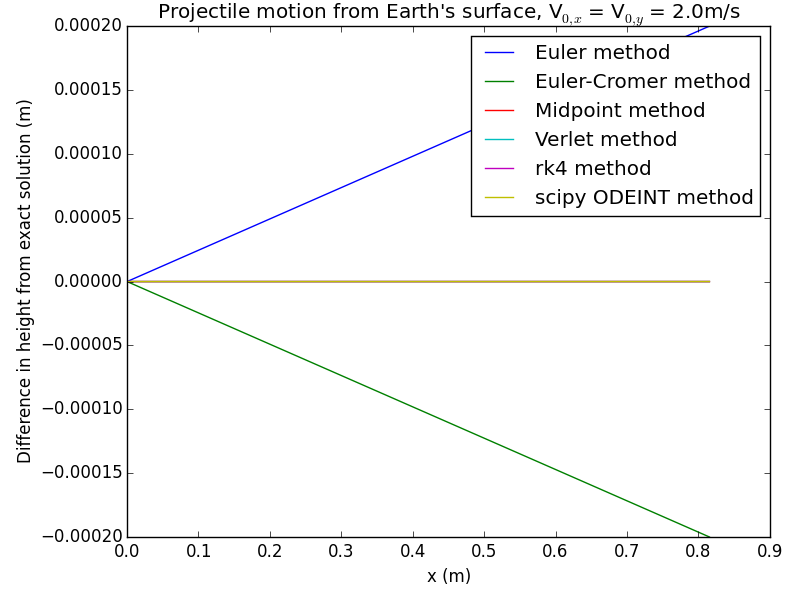
\includegraphics[scale=0.6]{figures/test_cases/projectile_motion_difference_from_exact_all_methods.png}
\caption{Difference between calculated heights and exact height for each integration method against x distance for projectile being launched from Earth's surface with $V_x = V_y = 2.0$m/s.}\label{fig:projectile_motion_difference_from_exact_all_methods}
\end{figure}

It is clear to see here that the Euler method and Euler-Cromer method fail to follow the exact solution compared to the other methods, which agree with the exact solution closer. The following figure \ref{fig:projectile_motion_difference_from_exact_good_methods} shows the same plot as figure \ref{fig:projectile_motion_difference_from_exact_all_methods} except it only includes the Midpoint method, Verlet method, RK4 method, and scipy ODEINT method, excluding the Euler and Euler-Cromer methods.\\

\begin{figure}[!htb]
\centering
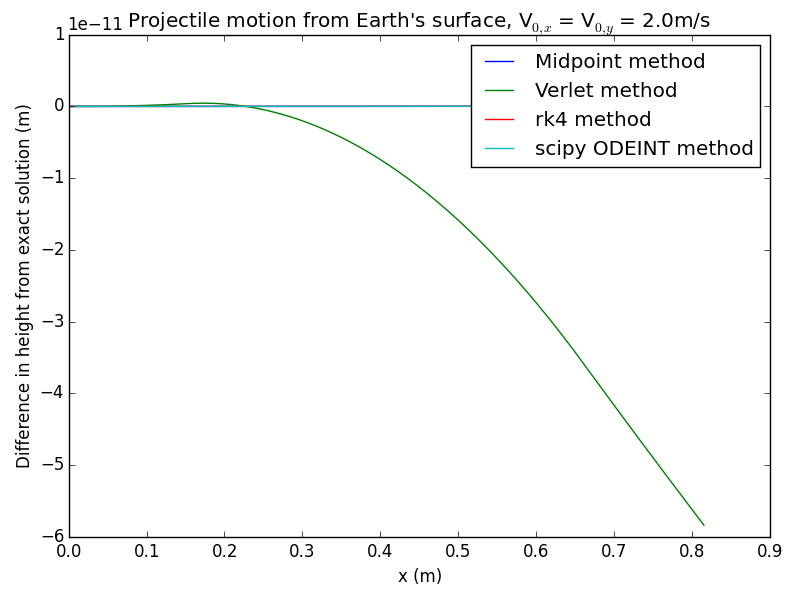
\includegraphics[scale=0.6]{figures/test_cases/projectile_motion_difference_from_exact_good_methods.png}
\caption{Difference between calculated heights and exact height for each integration method against x distance for projectile being launched from Earth's surface with $V_x = V_y = 2.0$m/s.}\label{fig:projectile_motion_difference_from_exact_good_methods}
\end{figure}

Each of these methods very closely agree with the exact solution, however the Midpoint method, RK4 method, and scipy ODEINT method agree closer to the exact solution than Verlet. The following figure \ref{fig:projectile_motion_difference_from_exact_good_methods_no_verlet} shows the same plot as the above two, except it only includes the Midpoint method, RK4 method, and scipy ODEINT method.\\

\begin{figure}[!htb]
\centering
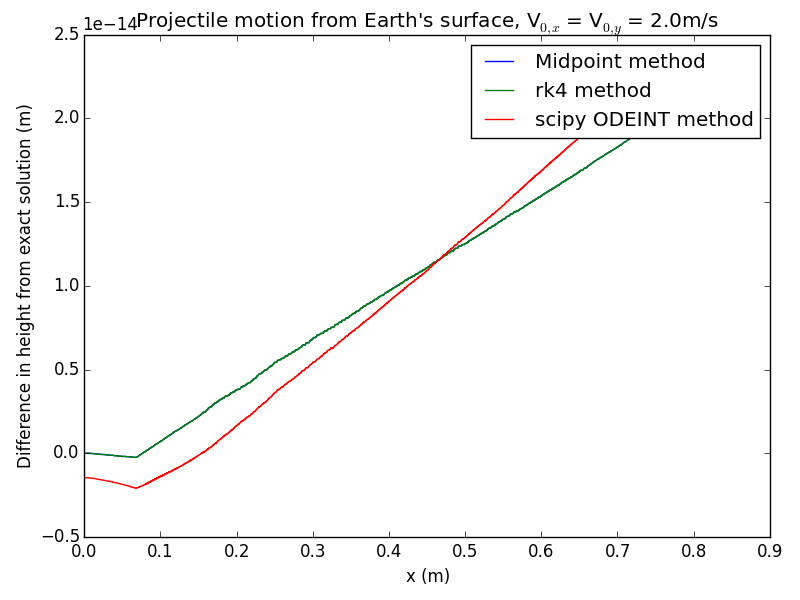
\includegraphics[scale=0.6]{figures/test_cases/projectile_motion_difference_from_exact_good_methods_no_verlet.png}
\caption{Difference between calculated heights and exact height for each integration method against x distance for projectile being launched from Earth's surface with $V_x = V_y = 2.0$m/s.}\label{fig:projectile_motion_difference_from_exact_good_methods_no_verlet}
\end{figure}

Similarly, the above figures were plotted for a projectile being launched from the earth's surface with $V_x = 2.0$m/s, $V_y = V_{escape}$ and shown in figures \ref{fig:projectile_motion_escape_velocity_difference_from_exact_all_methods} and \ref{fig:projectile_motion_escape_velocity_difference_from_exact_good_methods}.\\

\begin{figure}[!htb]
\centering
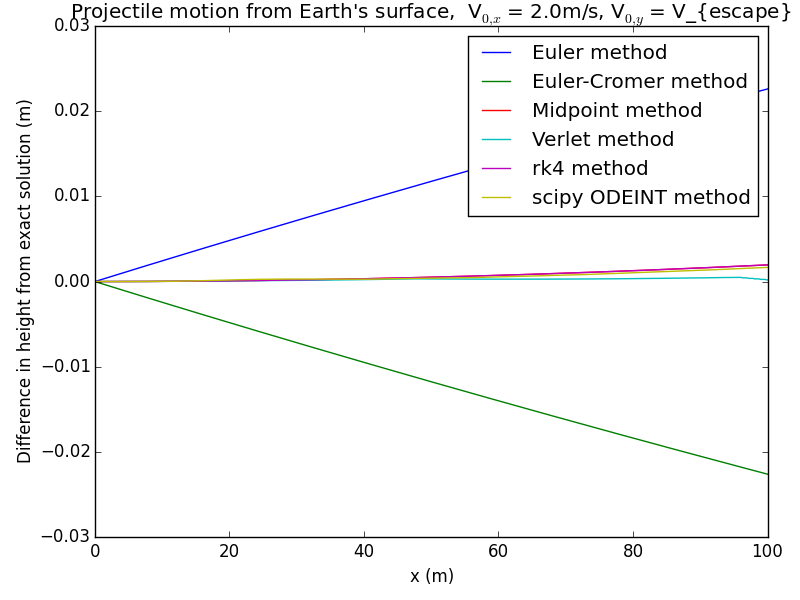
\includegraphics[scale=0.6]{figures/test_cases/projectile_motion_escape_velocity_difference_from_exact_all_methods.png}
\caption{Difference between calculated heights and exact height for each integration method against x distance for projectile being launched from Earth's surface with $V_x = 2.0$m/s and $V_y = V_{escape}$.}\label{fig:projectile_motion_escape_velocity_difference_from_exact_all_methods}
\end{figure}

\begin{figure}[!htb]
\centering
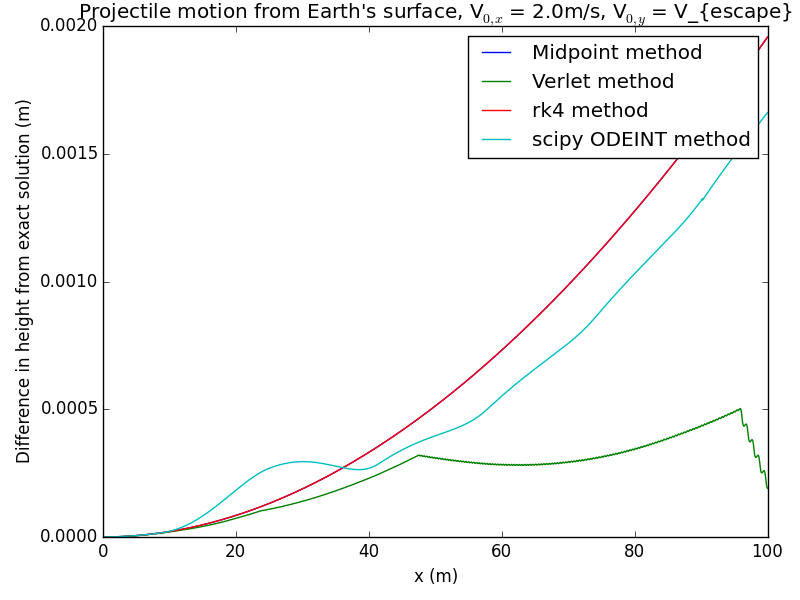
\includegraphics[scale=0.6]{figures/test_cases/projectile_motion_escape_velocity_difference_from_exact_good_methods.png}
\caption{Difference between calculated heights and exact height for each integration method against x distance for projectile being launched from Earth's surface with $V_x = 2.0$m/s and $V_y = V_{escape}$.}\label{fig:projectile_motion_escape_velocity_difference_from_exact_good_methods}
\end{figure}

The Midpoint method and RK4 method lie on top of one another. These are all very close to the exact result (down to a 1e-14 m difference for the case of $V_x = V_y = 2.0$m/s and down to 0.002 m difference for the case of  $V_x = 2.0$m/s and $V_y = V_{escape}$) and so each of these methods are viable candidates as they pass the projectile motion test.\\ 

\subsection{Moon's Orbit}

The second test involved simulating the orbit of the moon around the earth and plotting the energies of the orbit to test if the methods conserved energy. The velocity of the moon as well as it's distance to Earth is used to initialize the phase space coordinates of the moon and a single orbit around the earth (period of 27.373 days) is animated (see ``moon.mp4" file in animation folder for animation). The following figure \ref{fig:Energy_conservation_all_methods} shows the plots of the energies from each integration method's solution subtracted from the initial energy of the orbit calculated from the initial conditions.\\

\begin{figure}[!htb]
\centering
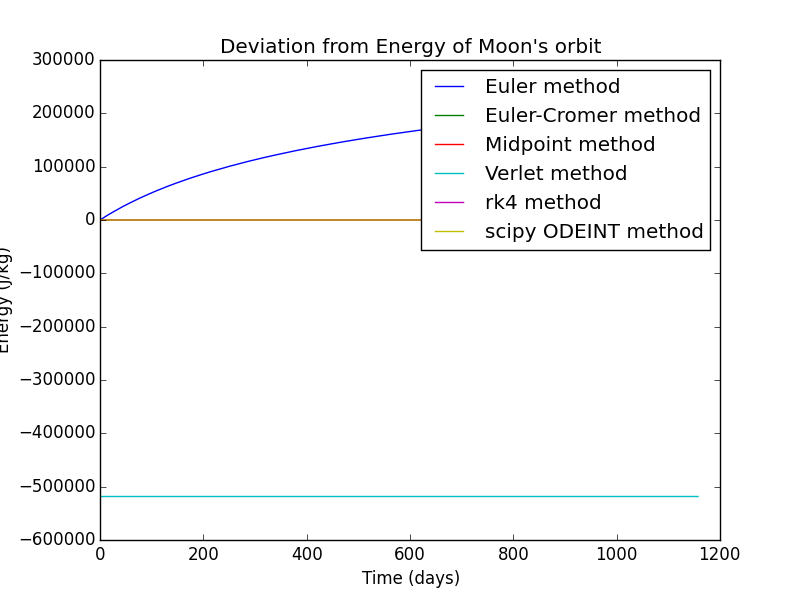
\includegraphics[scale=0.6]{figures/test_cases/Energy_conservation_all_methods.png}
\caption{Difference between calculated energies of Moon's orbit and exact initial energy for each integration method against time.}\label{fig:Energy_conservation_all_methods}
\end{figure}

The Euler method does not conserve energy, and the Verlet method calculates the wrong energy after the initial time step, so these methods are excluded and the following figure \ref{fig:Energy_conservation_good_methods} is produced of the remaining methods.\\

\begin{figure}[!htb]
\centering
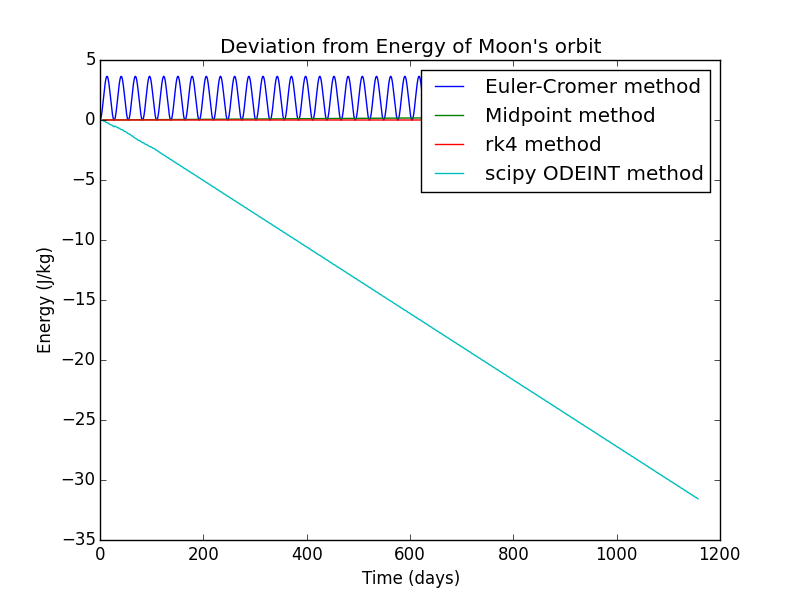
\includegraphics[scale=0.6]{figures/test_cases/Energy_conservation_good_methods.png}
\caption{Difference between calculated energies of Moon's orbit and exact initial energy for each integration method against time.}\label{fig:Energy_conservation_good_methods}
\end{figure}

The scipy ODEINT method does not conserve energy, and so it is excluded and the following figure \ref{fig:Energy_conservation_good_methods_no_ODEINT} is produced of the remaining methods.\\

\begin{figure}[!htb]
\centering
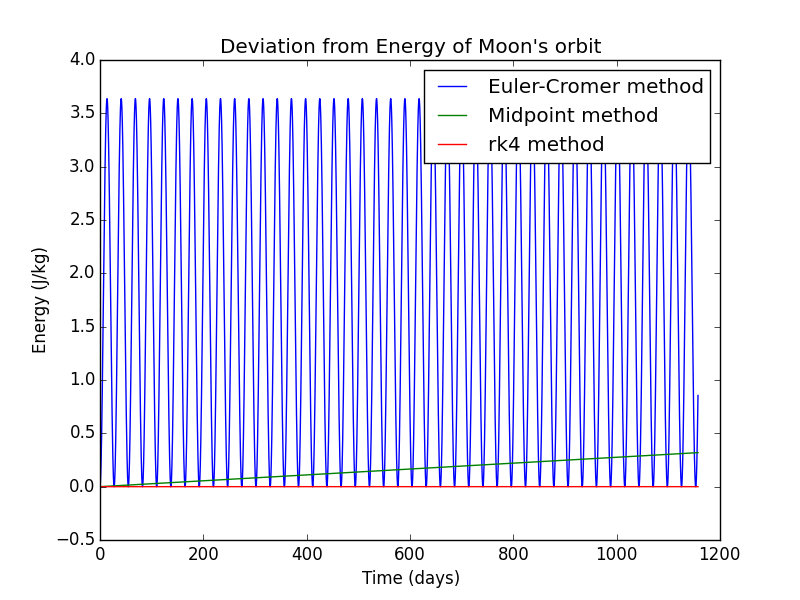
\includegraphics[scale=0.6]{figures/test_cases/Energy_conservation_good_methods_no_ODEINT.png}
\caption{Difference between calculated energies of Moon's orbit and exact initial energy for each integration method against time.}\label{fig:Energy_conservation_good_methods_no_ODEINT}
\end{figure}

Euler-Cromer has periodic fluctuations in the energies calculated, Midpoint method has energy increasing over time, albeit at a very slow pace, and the RK4 method seems to conserve energy throughout, measuring the exact initial energy of the orbit at all times with no fluctuations.\\

The only two methods that succeeded the above two tests were the Midpoint method and RK4 method. Both methods obtain the closest results to the analytic solution for both projectile motion tests. The Midpoint method conserves energy fairly well, although it has energy increasing slowly over time, while the RK4 method conserves energy throughout. Because of the above two tests, the RK4 method is chosen to be our integration method of choice as it successfully obtains expected, physical results.\\

\section{Simulations}

After an ODE solver method had been chosen (RK4) as it passed the above tests, the N-body simulations were be performed. Galaxy collisions, Lagrange points, and 3-body scattering were studied using the RK4 method of integration. The code for the simulations themselves can be found in the complementary python code under section 3) Simulations.\\

\subsection{Galaxy Collisions}

Various simulations of colliding two galaxies were performed at two different impact distances, a nearby collision in which the centre of each galaxy falls within the other's disk, and a far away collision in which the centre of each galaxy lies outside of the other's disk. The two galaxies have the following characteristics:\\

\begin{table}[!htb]
\centering
\begin{tabular}{|l|l|l|l|}
\hline
Galaxy	&	Mass (M$_\odot$)	&	Radius (kpc)	&	Initial position (x,y) (kpc)\\
\hline
$1$		&	$1 \times 10^{11}$	&	$30$			&	(0.0,0.0) \\
\hline
$2$ 	&	$1 \times 10^{10}$	& 	$15$			&	(70.71,70.71)\\ 
\hline
\end{tabular}
\caption{Characteristics of the two galaxies shared between each galaxy collision simulation.}\label{tab:galaxy_collision_characteristics}
\end{table}

Ten thousand stars are simulated in each galaxy. Stars in each galaxy are placed at random radial positions (within the radius of the galaxy) and random angular positions (from $0 \degree$ to $360 \degree$) such that each disk have randomly placed stars within their corresponding radius. The velocities of each star is set such that the stars orbit the galaxy in circular orbits at their position with respect to the centre of the galaxy. Each collision has the orbit of stars either orbiting clockwise or counter-clockwise, and the initial velocity of galaxy 2 set such that the impact distance between the galaxies is either within the disk of the first galaxy, or outside of the disk, and that the galaxies are on zero-energy, parabolic trajectories. Each collision starts with the above characteristics of each galaxy. The start of each collision appears as the below figure \ref{fig:galaxy_collision_initialized}.\\

\begin{figure}[!htb]
\centering
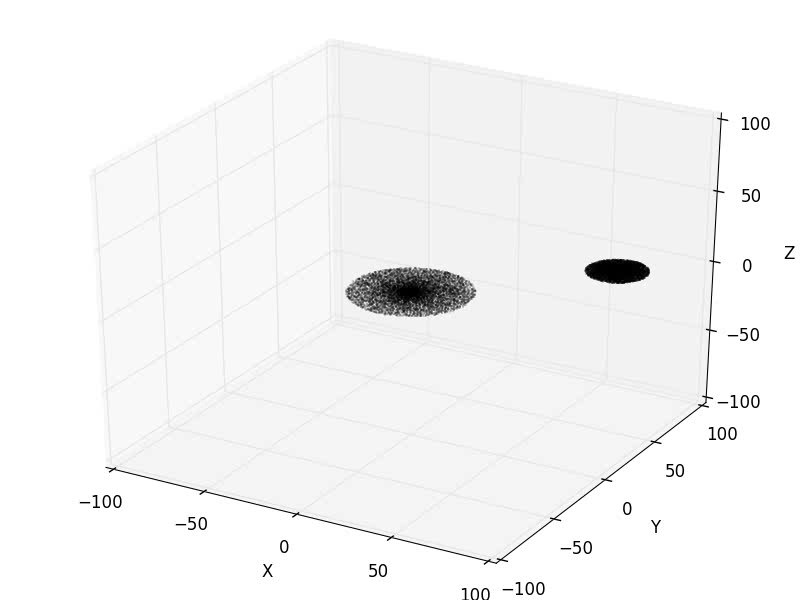
\includegraphics[scale=0.55]{figures/galaxy_collisions/galaxy_collision_initialized.png}
\caption{Starting positions of each galaxy collision simulation.}\label{fig:galaxy_collision_initialized}
\end{figure}

The following figure \ref{fig:rk4_parabolic_orbit_10000_particles_counterclockwise} shows the impact of two galaxies with their stars' orbital angular momenta aligned with the angular momentum of the colliding galaxies, and with a closest approach of the two galaxies set such that the centres of each galaxy lie within the other's disk (close approach).\\

\begin{figure}[!htb]
\minipage{0.5\textwidth}
  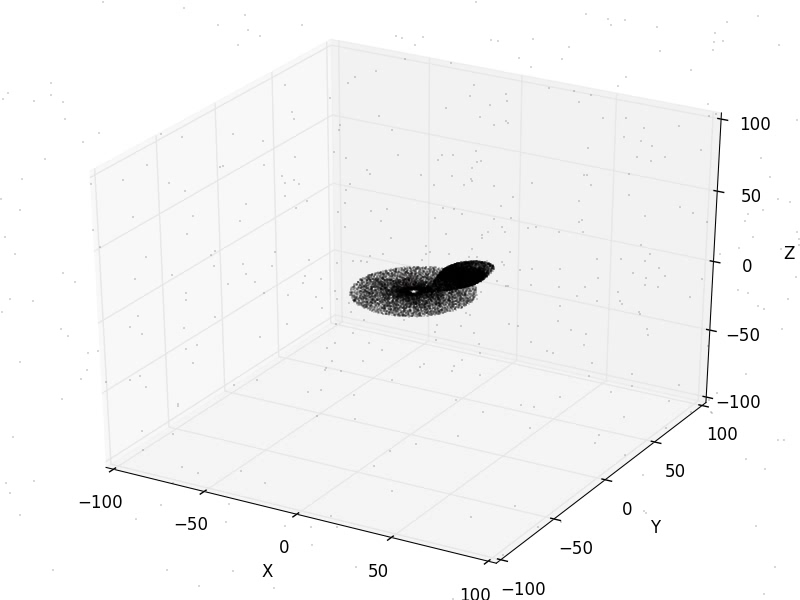
\includegraphics[width=\linewidth]{figures/galaxy_collisions/rk4_parabolic_orbit_10000_particles_counterclockwise_fig1.png}
  \subcaption{}\label{fig:rk4_parabolic_orbit_10000_particles_counterclockwise_fig1}
\endminipage\hfill
\minipage{0.5\textwidth}
  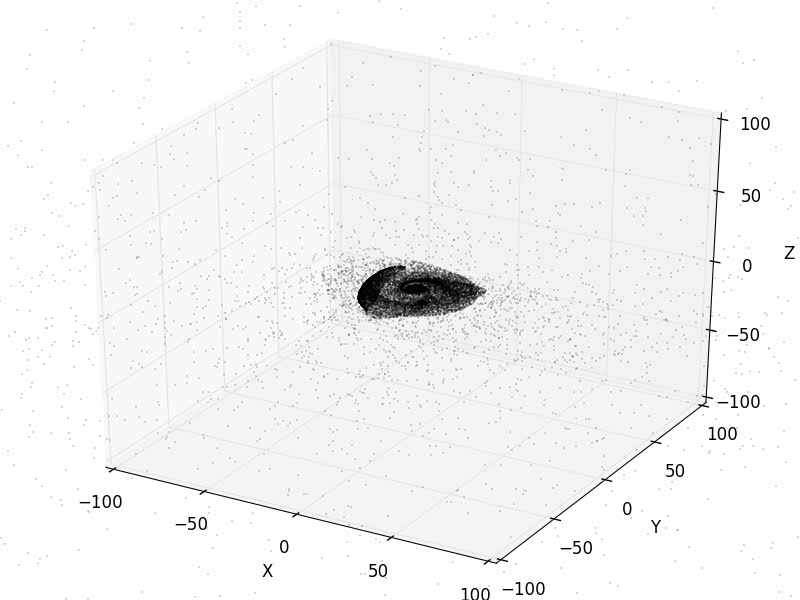
\includegraphics[width=\linewidth]{figures/galaxy_collisions/rk4_parabolic_orbit_10000_particles_counterclockwise_fig2.png}
  \subcaption{}\label{fig:rk4_parabolic_orbit_10000_particles_counterclockwise_fig2}
\endminipage\hfill
\minipage{0.5\textwidth}%
  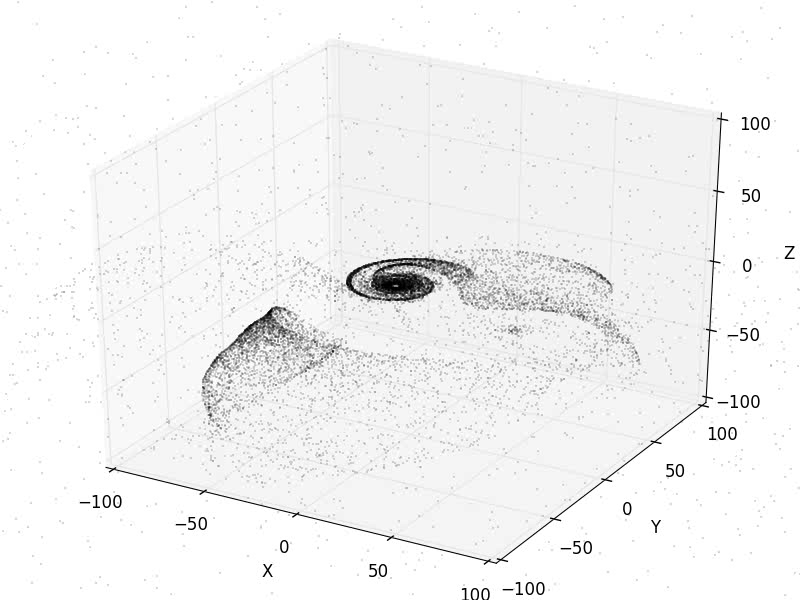
\includegraphics[width=\linewidth]{figures/galaxy_collisions/rk4_parabolic_orbit_10000_particles_counterclockwise_fig3.png}
  \subcaption{}\label{fig:rk4_parabolic_orbit_10000_particles_counterclockwise_fig3}
\endminipage
\minipage{0.5\textwidth}%
  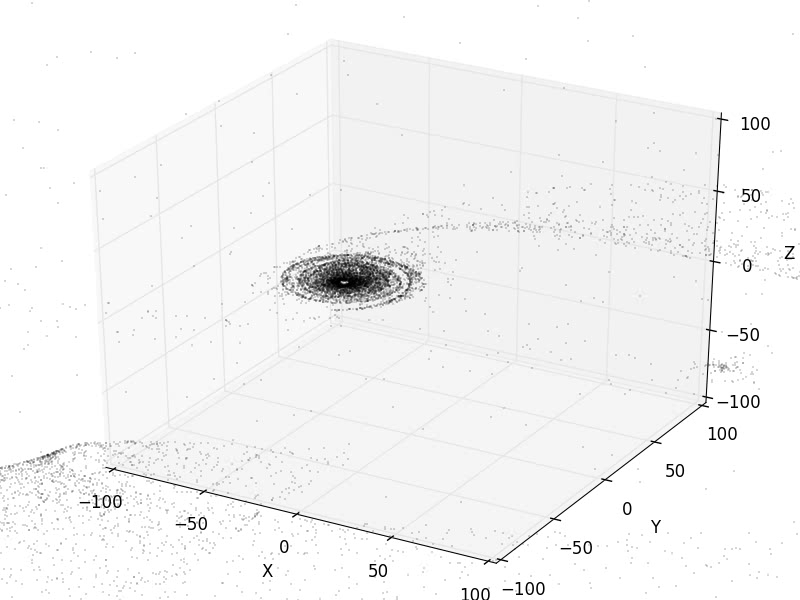
\includegraphics[width=\linewidth]{figures/galaxy_collisions/rk4_parabolic_orbit_10000_particles_counterclockwise_fig4.png}
  \subcaption{}\label{fig:rk4_parabolic_orbit_10000_particles_counterclockwise_fig4}
\endminipage
\caption{Collision of two galaxies with the stars' orbital angular momenta aligned with the angular momentum of the collision, close approach. (\ref{fig:rk4_parabolic_orbit_10000_particles_counterclockwise_fig1}) Pre-collision. (\ref{fig:rk4_parabolic_orbit_10000_particles_counterclockwise_fig2}) Collision. (\ref{fig:rk4_parabolic_orbit_10000_particles_counterclockwise_fig3}) Post-collision. (\ref{fig:rk4_parabolic_orbit_10000_particles_counterclockwise_fig4})
Post-collision, long term.}\label{fig:rk4_parabolic_orbit_10000_particles_counterclockwise}
\end{figure}

During the pre-collision phase (figure \ref{fig:rk4_parabolic_orbit_10000_particles_counterclockwise_fig1}), the side of the disk of galaxy 2 nearest to the centre of galaxy 1 begins to accelerate towards the centre of galaxy 1 while still orbiting galaxy 2 counter-clockwise. This results in the disk of galaxy 2 elongating along an axis between the galaxies' radial separation and the positive x-axis towards the right of the centre of galaxy 1. During the collision phase (figure \ref{fig:rk4_parabolic_orbit_10000_particles_counterclockwise_fig2}), you can see the stars of galaxy 2, whose orbital velocities are along the direction of the velocity of galaxy 2 during the collision, begin to leave the two galaxies on the left side of the collision. These stars have gained a boost to their velocities such that they can escape the two galaxies. The rest of the stars wrap around galaxy 1 (as seen in the top right of the collision) or fall towards the center. During the post-collision phase (figure \ref{fig:rk4_parabolic_orbit_10000_particles_counterclockwise_fig3}), you can see the stars that were on the left side of the collision of figure \ref{fig:rk4_parabolic_orbit_10000_particles_counterclockwise_fig2} that were stripped from galaxy 2 leave the two galaxies, escaping the system, as well as the stars that were on the top right side of the collision that were also stripped from galaxy 2 leave the two galaxies, escaping the system towards the right of the simulation. Some of the stars on the right side come from galaxy 2 perturbing the disk of galaxy 1, causing stars in galaxy 1 to gain energy as galaxy 2 leaves the collision, resulting in them leaving the disk of galaxy 1, wrap around galaxy 1, and fall in towards the centre of galaxy 1, producing long arms with the stripped stars of galaxy 2 on the right. Galaxy 2 is mostly stripped as it leaves the collision, with only a few stars close to the centre of the galaxy still orbiting it. During the post-collision, long term phase (figure \ref{fig:rk4_parabolic_orbit_10000_particles_counterclockwise_fig4}), galaxy 2 has reached the edge of the simulation, along with the stars on the left side that had their velocity's boosted, while the stars whose orbits were perturbed by galaxy 2 on the right side continue to fall into galaxy 1 in a long arm, or escape. Galaxy 1's disk has perturbed such that spiral arm-like structures have formed and are now winding up in a counter-clockwise direction.\\

The following figure \ref{fig:rk4_parabolic_orbit_10000_particles_clockwise} shows the impact of two galaxies with their stars' orbital angular momenta opposite to the angular momentum of the colliding galaxies, and with a closest approach of the two galaxies set such that the centres of each galaxy lie within the other's disk (close approach).\\

\begin{figure}[!htb]
\minipage{0.5\textwidth}
  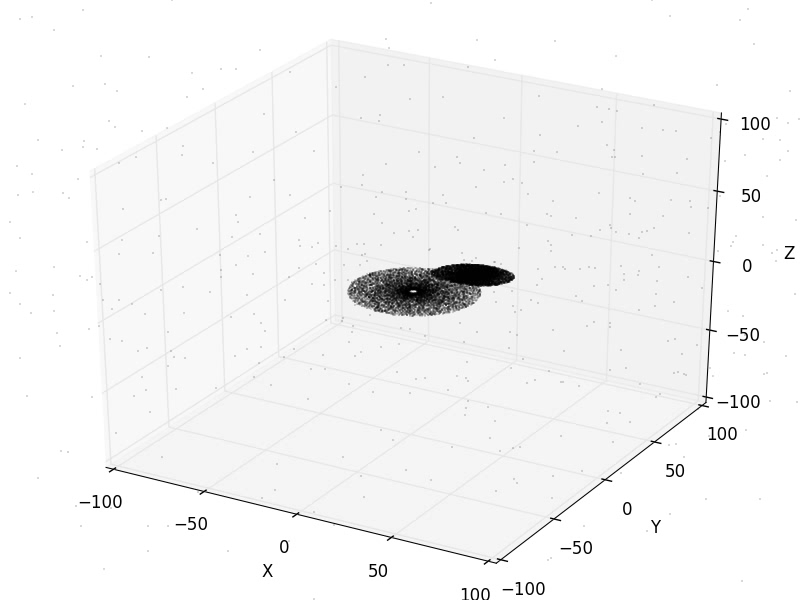
\includegraphics[width=\linewidth]{figures/galaxy_collisions/rk4_parabolic_orbit_10000_particles_clockwise_fig1.png}
  \subcaption{}\label{fig:rk4_parabolic_orbit_10000_particles_clockwise_fig1}
\endminipage\hfill
\minipage{0.5\textwidth}
  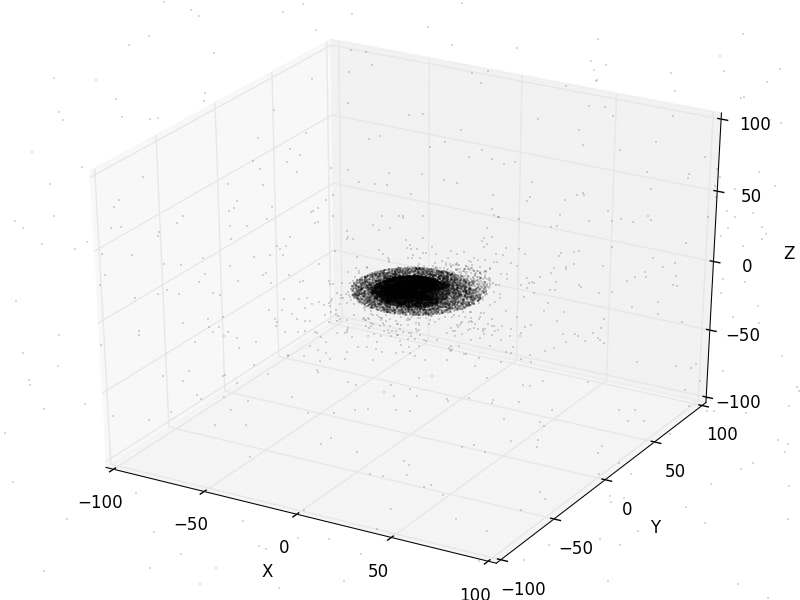
\includegraphics[width=\linewidth]{figures/galaxy_collisions/rk4_parabolic_orbit_10000_particles_clockwise_fig2.png}
  \subcaption{}\label{fig:rk4_parabolic_orbit_10000_particles_clockwise_fig2}
\endminipage\hfill
\minipage{0.5\textwidth}%
  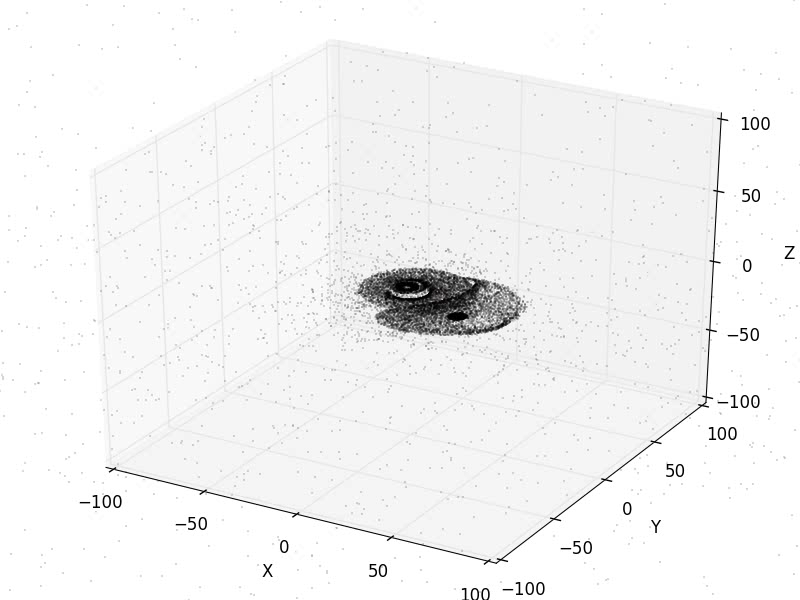
\includegraphics[width=\linewidth]{figures/galaxy_collisions/rk4_parabolic_orbit_10000_particles_clockwise_fig3.png}
  \subcaption{}\label{fig:rk4_parabolic_orbit_10000_particles_clockwise_fig3}
\endminipage
\minipage{0.5\textwidth}%
  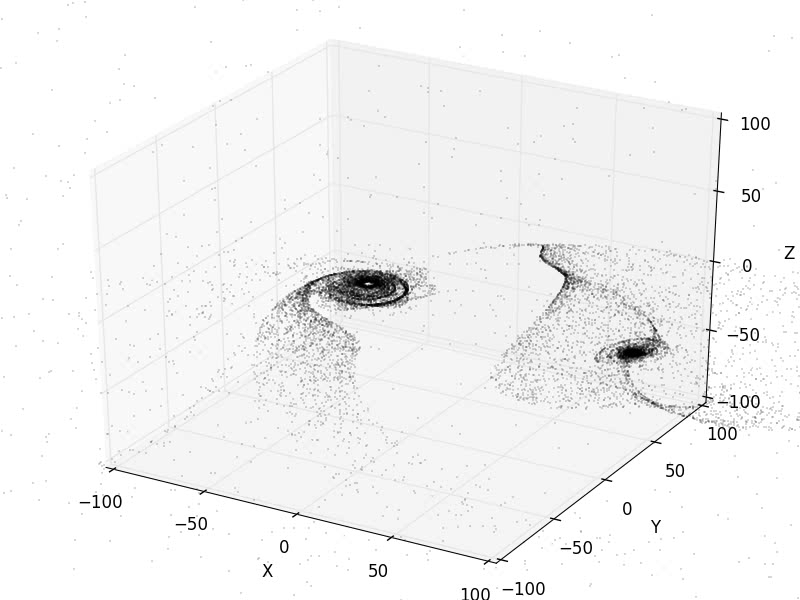
\includegraphics[width=\linewidth]{figures/galaxy_collisions/rk4_parabolic_orbit_10000_particles_clockwise_fig4.png}
  \subcaption{}\label{fig:rk4_parabolic_orbit_10000_particles_clockwise_fig4}
\endminipage
\caption{Collision of two galaxies with the stars' orbital angular momenta opposite to the angular momentum of the collision, close approach. (\ref{fig:rk4_parabolic_orbit_10000_particles_clockwise_fig1}) Pre-collision. (\ref{fig:rk4_parabolic_orbit_10000_particles_clockwise_fig2}) Collision. (\ref{fig:rk4_parabolic_orbit_10000_particles_clockwise_fig3}) Post-collision. (\ref{fig:rk4_parabolic_orbit_10000_particles_clockwise_fig4})
Post-collision, long term.}\label{fig:rk4_parabolic_orbit_10000_particles_clockwise}
\end{figure}

During the pre-collision phase (figure \ref{fig:rk4_parabolic_orbit_10000_particles_clockwise_fig1}), the disk of galaxy 2 no longer elongates along an axis between the galaxies' radial separation and positive x-axis as in figure \ref{fig:rk4_parabolic_orbit_10000_particles_counterclockwise_fig1}, but instead along an axis between the galaxies' radial separation and negative x-axis. This is due to that fact that the stars of galaxy 2 closest to the centre of galaxy 1 are accelerated towards the centre of galaxy 1 as they orbit galaxy 2 in a clockwise direction. During the collision phase (figure \ref{fig:rk4_parabolic_orbit_10000_particles_clockwise_fig2}), the stars of galaxy 2 begin to wrap around galaxy 1 while galaxy 2's disk begins to perturb. During the post-collision phase (figure \ref{fig:rk4_parabolic_orbit_10000_particles_clockwise_fig3}), the stars of galaxy 1 have their velocity's boosted along the direction tangential to the velocity of the centre of galaxy 2. However, since the stars' orbital angular momenta and the angular momentum of the collision are opposite, the stars on the right side instead gain a boost to their velocity's such that they can escape, and as they leave in the same direction as galaxy 2 and the rest of the stars do not gain enough velocity to escape, the general shape of galaxy 2 remains relatively the same compared to figure \ref{fig:rk4_parabolic_orbit_10000_particles_counterclockwise_fig3}.  During the post-collision, long term phase (figure \ref{fig:rk4_parabolic_orbit_10000_particles_clockwise_fig4}), galaxy 1's disk has been perturbed by galaxy 2 to form spiral arm-like structures. Some stars in galaxy 1 have been boosted by galaxy 2 such that they leave the disk of galaxy 1 and form long arms that fall towards the centre of galaxy 1, as seen in the bottom left, in a similar fashion to the stars of galaxy 2 in the right side of figure \ref{fig:rk4_parabolic_orbit_10000_particles_counterclockwise_fig3}. Galaxy 2's disk has expanded, and some stars have starting falling towards the centre of galaxy 2 in spiral arm-like structures on opposite sides of galaxy 2. Galaxy 2 has not been as stripped as it was for the case of figure \ref{fig:rk4_parabolic_orbit_10000_particles_clockwise}. As in figure \ref{fig:rk4_parabolic_orbit_10000_particles_counterclockwise_fig4}, galaxy 1's disk has perturbed such that spiral arm-like structures have formed and are now winding up in a clockwise direction.\\

The following figure \ref{fig:rk4_parabolic_orbit_10000_particles_counterclockwise_velx_escape} shows the impact of two galaxies with their stars' orbital angular momenta aligned with the angular momentum of the colliding galaxies, and with a closest approach of the two galaxies set such that the centres of each galaxy lie outside the other's disk (far approach).\\

\begin{figure}[!htb]
\minipage{0.5\textwidth}
  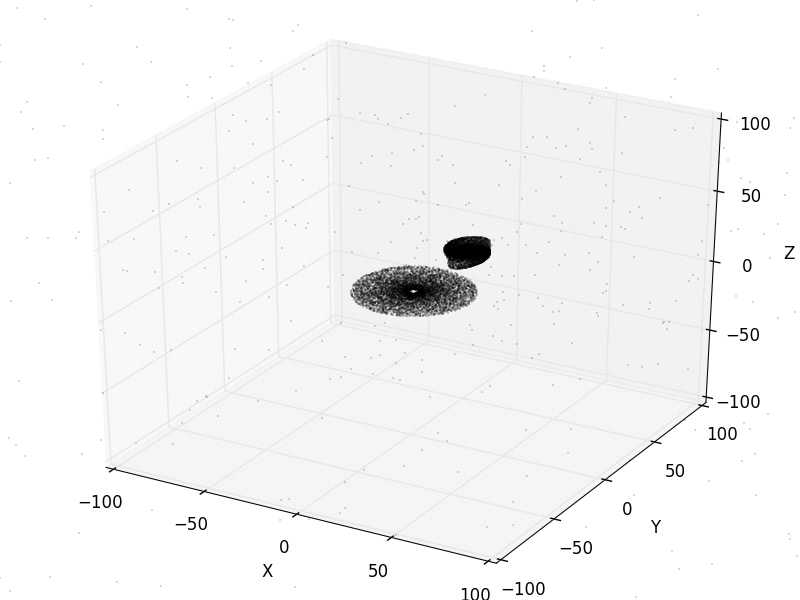
\includegraphics[width=\linewidth]{figures/galaxy_collisions/rk4_parabolic_orbit_10000_particles_counterclockwise_velx_escape_fig1.png}
  \subcaption{}\label{fig:rk4_parabolic_orbit_10000_particles_counterclockwise_velx_escape_fig1}
\endminipage\hfill
\minipage{0.5\textwidth}
  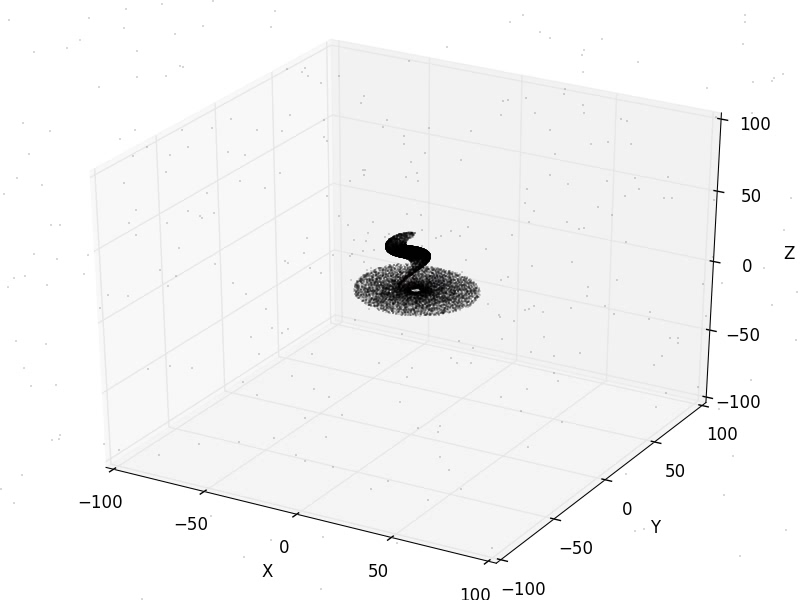
\includegraphics[width=\linewidth]{figures/galaxy_collisions/rk4_parabolic_orbit_10000_particles_counterclockwise_velx_escape_fig2.png}
  \subcaption{}\label{fig:rk4_parabolic_orbit_10000_particles_counterclockwise_velx_escape_fig2}
\endminipage\hfill
\minipage{0.5\textwidth}%
  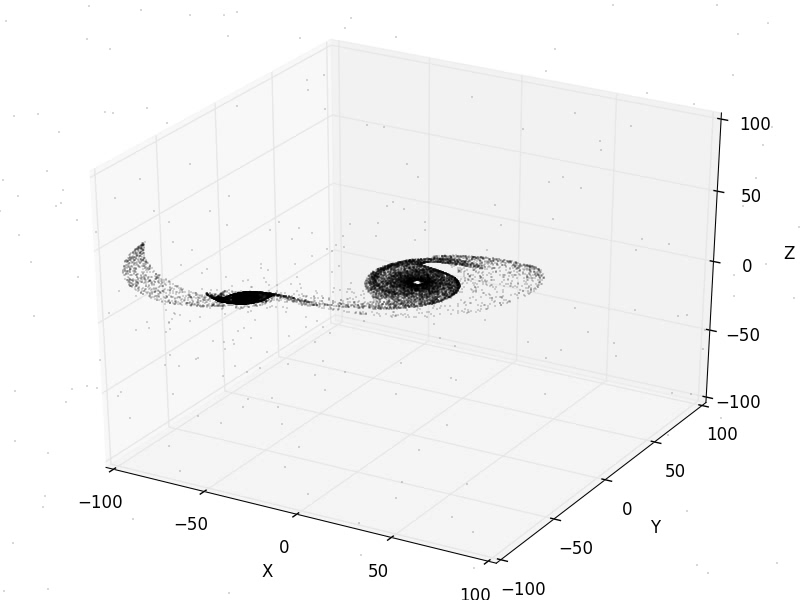
\includegraphics[width=\linewidth]{figures/galaxy_collisions/rk4_parabolic_orbit_10000_particles_counterclockwise_velx_escape_fig3.png}
  \subcaption{}\label{fig:rk4_parabolic_orbit_10000_particles_counterclockwise_velx_escape_fig3}
\endminipage
\minipage{0.5\textwidth}%
  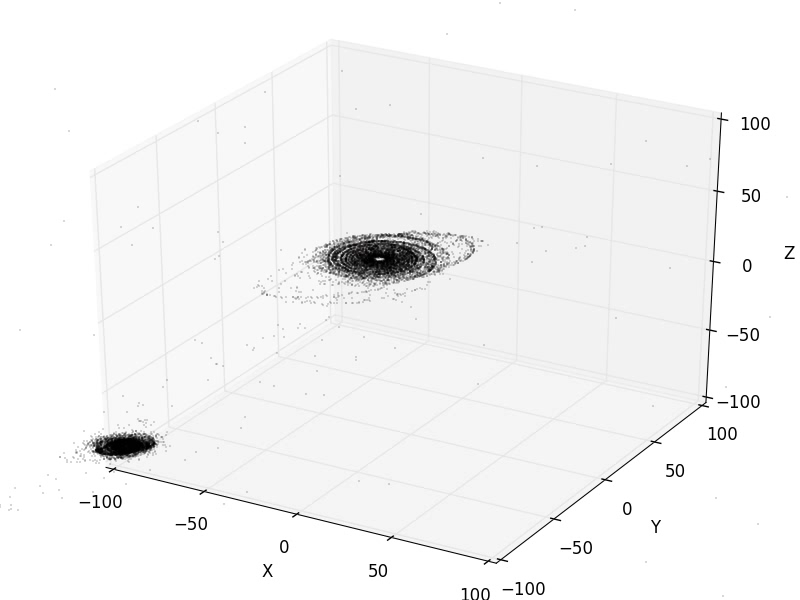
\includegraphics[width=\linewidth]{figures/galaxy_collisions/rk4_parabolic_orbit_10000_particles_counterclockwise_velx_escape_fig4.png}
  \subcaption{}\label{fig:rk4_parabolic_orbit_10000_particles_counterclockwise_velx_escape_fig4}
\endminipage
\caption{Collision of two galaxies with the stars' orbital angular momenta aligned with the angular momentum of the collision, far approach. (\ref{fig:rk4_parabolic_orbit_10000_particles_counterclockwise_velx_escape_fig1}) Pre-collision. (\ref{fig:rk4_parabolic_orbit_10000_particles_counterclockwise_velx_escape_fig2}) Closest approach. (\ref{fig:rk4_parabolic_orbit_10000_particles_counterclockwise_velx_escape_fig3}) Post-collision. (\ref{fig:rk4_parabolic_orbit_10000_particles_counterclockwise_velx_escape_fig4})
Post-collision, long term.}\label{fig:rk4_parabolic_orbit_10000_particles_counterclockwise_velx_escape}
\end{figure}

During the pre-collision phase (figure \ref{fig:rk4_parabolic_orbit_10000_particles_counterclockwise_velx_escape_fig1}), the side of the disk of galaxy 2 nearest to the centre of galaxy 1 begins to accelerate towards the centre of galaxy 1. These stars lose their orbital velocities and begin to fall into galaxy 1, gaining velocities along the direction of the radial separation between the two galaxies. The side of the disk of galaxy 2 furthest from the centre of galaxy 1 is given a boost as galaxy 2 is boosted. This results in the disk of galaxy 2 to elongate along the radial separation of galaxy 1 and galaxy 2 in a ``S" shape. During the closest approach phase (figure \ref{fig:rk4_parabolic_orbit_10000_particles_counterclockwise_velx_escape_fig2}), galaxy 2 has been further stretched towards the centre of galaxy 1 in a stronger ``S" shape, creating a strong spiral arm-like structure. The arm closest to galaxy 1 reaches out towards the left of the centre of galaxy 1, resulting in these stars to start to wrap around galaxy 1 counter-clockwise as they are accelerated towards the centre of galaxy 1, falling into the disk of galaxy 1 in counter-clockwise orbits, or otherwise follow the trajectory of galaxy 2 if the stars are far enough away from galaxy 1. The stars in the arm furthest away from galaxy 1 are given a boost along the direction of the velocity of the centre of galaxy 2 as it travels around galaxy 1. The disk of galaxy 1 starts to perturb and stretch towards the centre of galaxy 2. During the post-collision phase (figure \ref{fig:rk4_parabolic_orbit_10000_particles_counterclockwise_velx_escape_fig3}), on the left are the stars that were in the furthest arm from galaxy 1 and were given a boost as seen in figure \ref{fig:rk4_parabolic_orbit_10000_particles_counterclockwise_velx_escape_fig2}, some of them gain enough energy to escape galaxy 2, others fall back into galaxy 2, forming a long spiral arm-like structure. The stars that were in the arm closest to galaxy 1's centre are falling into either galaxy 1 or galaxy 2. A similar effect is occurring to galaxy 1's stars as galaxy 2's stars, except galaxy 1's stars on the arm furthest from galaxy 2 are not given enough of a boost to escape as galaxy 1 is not given a large enough boost after the collision, unlike galaxy 2. The stars in the arm emerging from galaxy 1 closest to galaxy 2 also are either falling into galaxy 1 or galaxy 2 after their orbits have been perturbed, but mostly are falling into galaxy 1 as galaxy 2's gravitational pull is weaker. During the post-collision, long term phase (figure \ref{fig:rk4_parabolic_orbit_10000_particles_counterclockwise_velx_escape_fig4}), the long arms of galaxy 2 have fallen into either galaxy 1 or galaxy 2 or escaped the system so they're no longer visible. The same effect is observed for the long arms of galaxy 1. Galaxy 2 appears stripped slightly. Smaller spiral arm-like structures are apparent in galaxy 1 and are winding up counter-clockwise.\\

The following figure \ref{fig:rk4_parabolic_orbit_10000_particles_clockwise_velx_escape} shows the impact of two galaxies with their stars' orbital angular momenta opposite to the angular momentum of the colliding galaxies, and with a closest approach of the two galaxies set such that the centres of each galaxy lie outside the other's disk (far approach).\\

\begin{figure}[!htb]
\minipage{0.5\textwidth}
  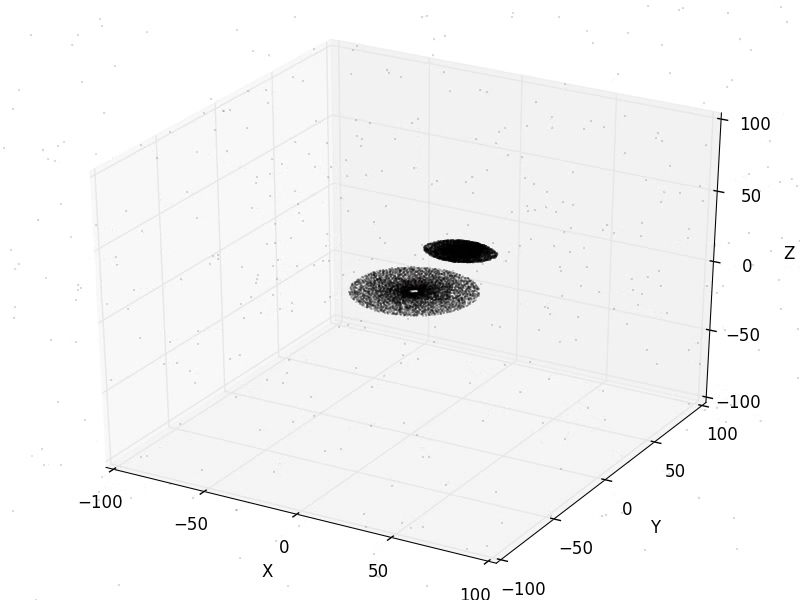
\includegraphics[width=\linewidth]{figures/galaxy_collisions/rk4_parabolic_orbit_10000_particles_clockwise_velx_escape_fig1.png}
  \subcaption{}\label{fig:rk4_parabolic_orbit_10000_particles_clockwise_velx_escape_fig1}
\endminipage\hfill
\minipage{0.5\textwidth}
  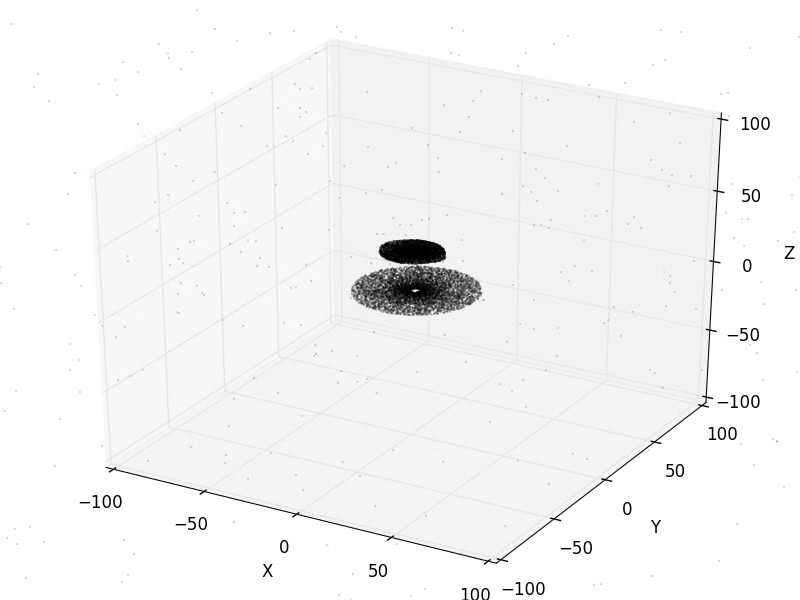
\includegraphics[width=\linewidth]{figures/galaxy_collisions/rk4_parabolic_orbit_10000_particles_clockwise_velx_escape_fig2.png}
  \subcaption{}\label{fig:rk4_parabolic_orbit_10000_particles_clockwise_velx_escape_fig2}
\endminipage\hfill
\minipage{0.5\textwidth}%
  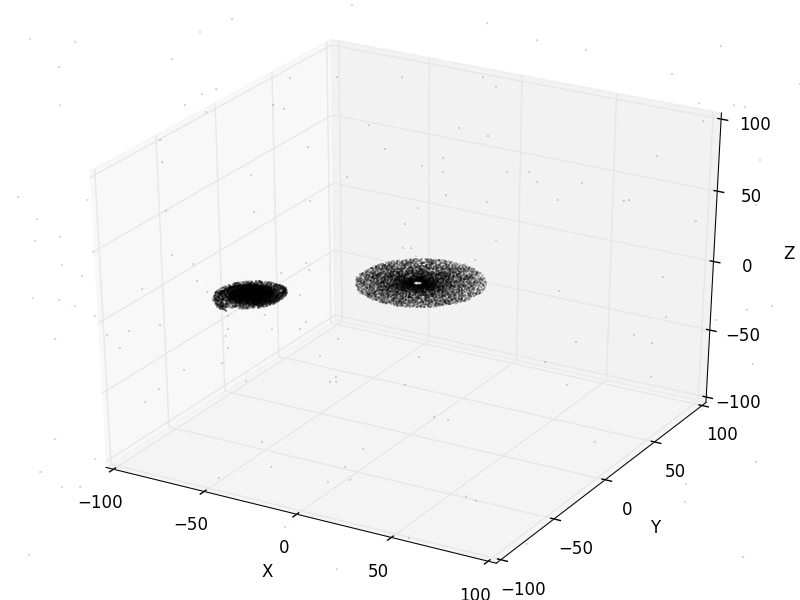
\includegraphics[width=\linewidth]{figures/galaxy_collisions/rk4_parabolic_orbit_10000_particles_clockwise_velx_escape_fig3.png}
  \subcaption{}\label{fig:rk4_parabolic_orbit_10000_particles_clockwise_velx_escape_fig3}
\endminipage
\minipage{0.5\textwidth}%
  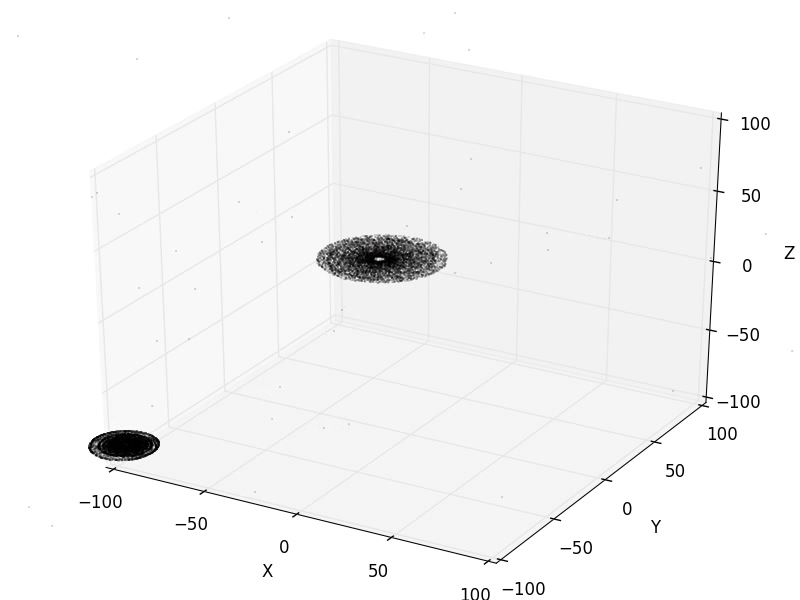
\includegraphics[width=\linewidth]{figures/galaxy_collisions/rk4_parabolic_orbit_10000_particles_clockwise_velx_escape_fig4.png}
  \subcaption{}\label{fig:rk4_parabolic_orbit_10000_particles_clockwise_velx_escape_fig4}
\endminipage
\caption{Collision of two galaxies with the stars' orbital angular momenta opposite to the angular momentum of the collision, far approach. (\ref{fig:rk4_parabolic_orbit_10000_particles_clockwise_velx_escape_fig1}) Pre-collision. (\ref{fig:rk4_parabolic_orbit_10000_particles_clockwise_velx_escape_fig2}) Closest approach. (\ref{fig:rk4_parabolic_orbit_10000_particles_clockwise_velx_escape_fig3}) Post-collision. (\ref{fig:rk4_parabolic_orbit_10000_particles_clockwise_velx_escape_fig4})
Post-collision, long term.}\label{fig:rk4_parabolic_orbit_10000_particles_clockwise_velx_escape}
\end{figure}

During the pre-collision phase (figure \ref{fig:rk4_parabolic_orbit_10000_particles_clockwise_velx_escape_fig1}), the side of the disk of galaxy 2 nearest to the centre of galaxy 1 begins to accelerate towards the centre of galaxy 1 as the stars orbit clockwise. This causes the arms to appear to elongate along an axis between the galaxies' radial separation and negative x-axis. Galaxy 1's disk appears slightly perturbed as it appears to be stretched along the x-axis. During the closest approach phase (figure \ref{fig:rk4_parabolic_orbit_10000_particles_clockwise_velx_escape_fig2}),  the stars at the left side of the disk of galaxy 2 slow down as they are accelerated towards the centre of galaxy 1, while the stars on the right speed up, resulting in the disk of galaxy 2 to further stretch. Galaxy 1's disk appears to be stretched along an axis perpendicular to the galaxies' radial separation. During the post-collision phase (figure \ref{fig:rk4_parabolic_orbit_10000_particles_clockwise_velx_escape_fig3}), on the bottom left of galaxy 2 are the stars that were sped up as they were accelerated towards galaxy 1 as seen in figure \ref{fig:rk4_parabolic_orbit_10000_particles_clockwise_velx_escape_fig2}. These stars were given a boost along their orbit and as such their orbits have grown, but only slightly a it was a small boost since there was only a small window where galaxy 1 gave a boost to these stars. On the top right of galaxy 1 are the stars that were slowed down by galaxy 1 as seen in figure \ref{fig:rk4_parabolic_orbit_10000_particles_clockwise_velx_escape_fig2}, now being sped up as the force due to galaxy 1 is along the same direction as their orbital velocities. This results in the short spiral arm-like structures emerging from the bottom left and top right parts of galaxy 2. During the post-collision, long term phase (figure \ref{fig:rk4_parabolic_orbit_10000_particles_clockwise_velx_escape_fig4}), the small arms of galaxy 2 have fallen into galaxy 2. There appears to be a dense region of stars on the outer edge of the disk of galaxy 2, as well as at the centre of the disk, separated by a less dense region of stars. Smaller spiral arm-like structures are apparent in galaxy 1 and are winding up clockwise. These spiral arms are much less prominent than the other galaxy collisions. There is no stripping of stars in this collision.\\

The results of the collision depend on the stars' orbital angular momentum and the angular momentum of the collision. When the orbital angular momentum and angular momentum of the collision are aligned, the collisions are more violent and result in more stripping of galaxy 2's stars as it passes by.\\
\pagebreak
\subsection{Lagrange Points}
Various simulations of the Lagrange points for the Sun-Earth were preformed in order to study the dynamics and stability of objects within these orbits. The orbits of all five Lagrange points were simulated, however the L2 and L4 points were the main area of focus for this project in terms of their stability at equilibrium and under a change in momentum. The plots in this section have their origins located at the centre of mass of the Sun-Earth system and the orbits are designed such that they are perfectly circular. The relevant initial conditions for all of these bodies are given as: \\

\begin{table}[!htb]
\centering
\begin{tabular}{|l|l|l|l|}
\hline
Object	&	Colour		&	Mass (M$_\odot$)			&	Initial position (x,y) (AU)\\
\hline
Sun		&	yellow		&	$1$							&	$\left(-\frac{M_\oplus}{M_\odot+M_\oplus}R, 0.0\right)$ \\
\hline
Earth 	&	blue		&	$3.003467 \times 10^{-6}$	&	$\left(\frac{M_\odot}{M_\odot+M_\oplus}R, 0.0\right)$ \\ 
\hline
$L_1$	&	red			&	$0$							& 	$\left(R\left[1-\left(\frac{1}{3}\frac{M_\odot}{M_\odot+M_\oplus}\right)^{1/3}\right],0.0\right)$ \\
\hline
$L_2$	&	green		&	$0$							& 	$\left(R\left[1+\left(\frac{1}{3}\frac{M_\odot}{M_\odot+M_\oplus}\right)^{1/3}\right],0.0\right)$ \\
\hline
$L_3$	&	cyan		&	$0$							& 	$\left(-R\left[1+\frac{5}{12}\frac{M_\odot}{M_\odot+M_\oplus}\right],0.0\right)$ \\
\hline
$L_4$	&	magenta		&	$0$							& 	$\left(\frac{R}{2}\frac{M_\odot-M_\oplus}{M_\odot+M_\oplus},\frac{\sqrt{3}}{2}R\right)$ \\
\hline
$L_5$	&	orange		&	$0$							& 	$\left(\frac{R}{2}\frac{M_\odot-M_\oplus}{M_\odot+M_\oplus},-\frac{\sqrt{3}}{2}R\right)$ \\
\hline
\end{tabular}
\caption{Characteristics of all the orbitting objects in the Lagrange point simulation.}\label{tab:lagrange_points_characteristics}
\end{table}

where $R$ is the constant distance separating the Sun and Earth (1 AU), and $M_\odot$ and $M_\oplus$ are the masses of the Sun and Earth respectively. The masses of all the objects placed in the Lagrange points are being neglected as they are small compared to the Sun-Earth system, and so effectively have zero mass. All the simulations begin in the following way, with the object initialized as the below figure \ref{fig:lagrange_points_initialized}.

\begin{figure}[!htb]
\centering
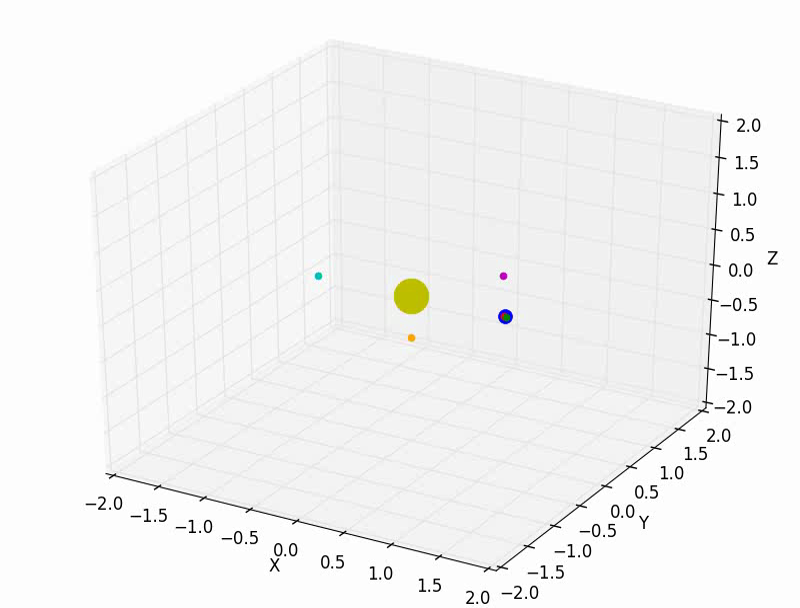
\includegraphics[scale=0.35]{figures/lagrange_points/lagrange_points_initialized.png}
\caption{Starting positions of all object in Lagrange point simulations.}\label{fig:lagrange_points_initialized}
\end{figure}

The L1 and L2 (red and green) points appear to be located within the radius of the Earth. This is due to the fact that the figure is scaled in terms of astronomical units and so the L1 and L2 points appear very close to Earth.\\ 

The stability of these orbits will be the main focus of this section and will be discussed by exploring figure \ref{fig:lagrange_points_stability}.

\begin{figure}[!htb]
\minipage{0.5\textwidth}
  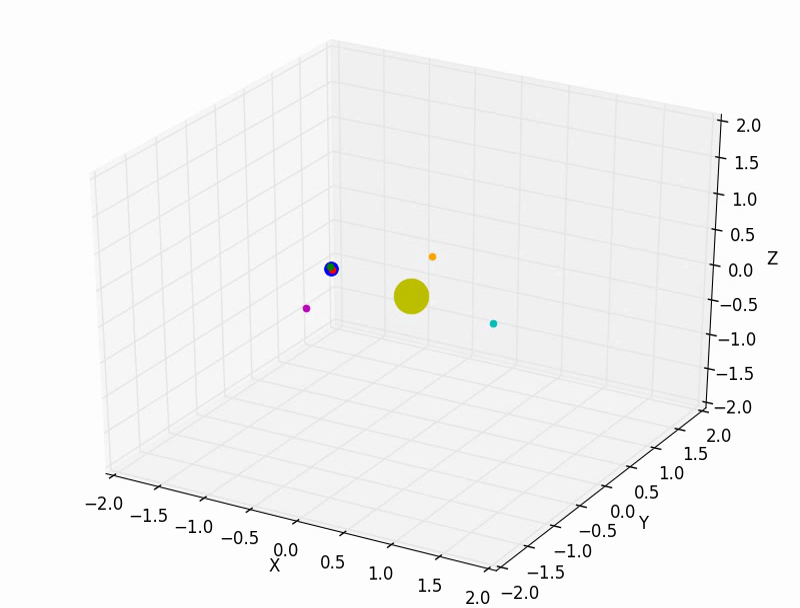
\includegraphics[width=\linewidth]{figures/lagrange_points/lagrange_points_stability_1.png}
  \subcaption{}\label{fig:lagrange_points_stability_fig1}
\endminipage\hfill
\minipage{0.5\textwidth}
  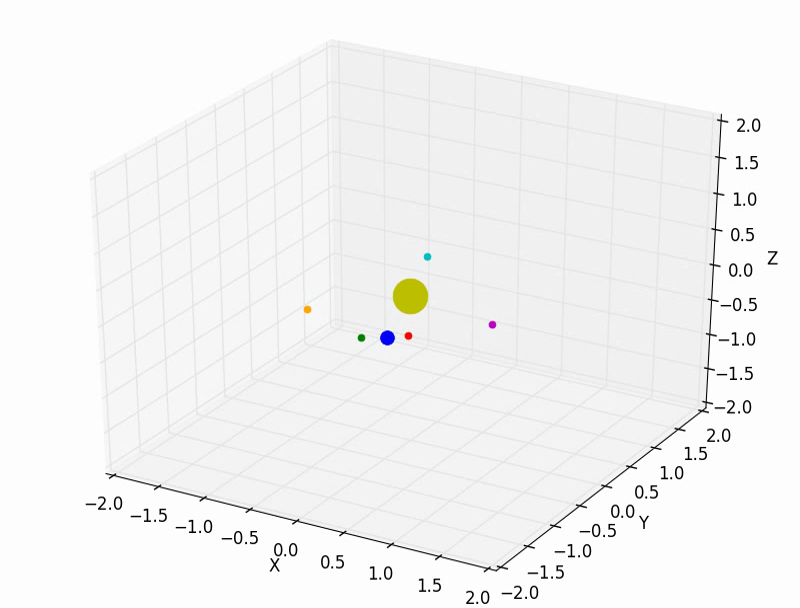
\includegraphics[width=\linewidth]{figures/lagrange_points/lagrange_points_stability_2.png}
  \subcaption{}\label{fig:lagrange_points_stability_fig2}
\endminipage\hfill
\minipage{0.5\textwidth}%
  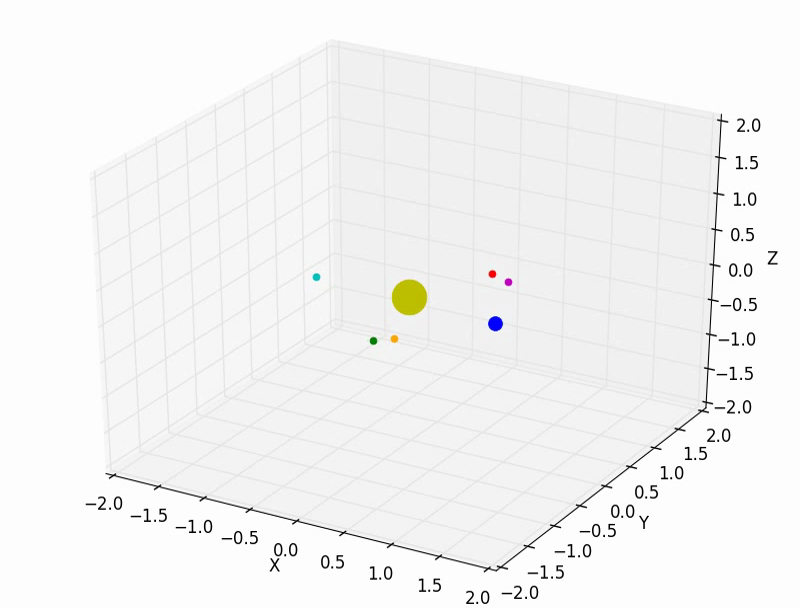
\includegraphics[width=\linewidth]{figures/lagrange_points/lagrange_points_stability_3.png}
  \subcaption{}\label{fig:lagrange_points_stability_fig3}
\endminipage
\minipage{0.5\textwidth}%
  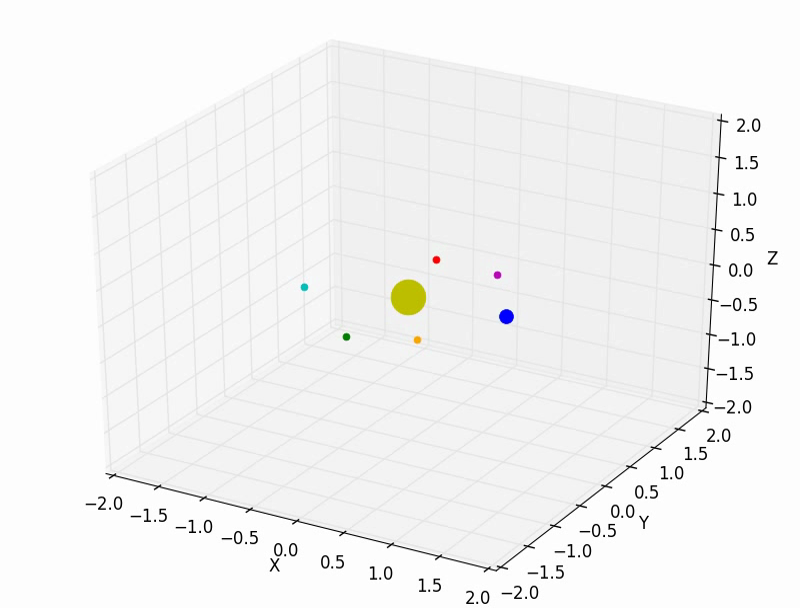
\includegraphics[width=\linewidth]{figures/lagrange_points/lagrange_points_stability_4.png}
  \subcaption{}\label{fig:lagrange_points_stability_fig4}
\endminipage
\caption{Orbits of the five Lagrange points of Sun-Earth system plotted over a time period of five years.
(\ref{fig:lagrange_points_stability_fig1}) Stable orbits. 
(\ref{fig:lagrange_points_stability_fig2}) Beginning of orbit drift. 
(\ref{fig:lagrange_points_stability_fig3}) Continued orbit drift. 
(\ref{fig:lagrange_points_stability_fig4}) End positions.}\label{fig:lagrange_points_stability}
\end{figure}

Throughout the duration of the first orbit (figure \ref{fig:lagrange_points_stability_fig1}) we can see that the object in at all the Lagrange points have maintained their initial positions relative to the Sun-Earth system. The L1 and L2 points have remained in orbit near the Earth, L3 has held its position on the opposite side of the Sun and the L4, L5 points have remained stable. We begin seeing deviations from the expected orbits a few months into the simulation (figure \ref{fig:lagrange_points_stability_fig2}). At this point we can see that the L1 point begins to lead the Earth orbit while the L2 point point begins lagging behind. We note that the L3 point is still located on the opposite side of the Sun and that the L4 and L5 points have not shown any sign of deviation. The orbits of the L1 and L2 points continue their drifting orbit (figure \ref{fig:lagrange_points_stability_fig3}), reaching almost the positions of the L4 and L5 points. It is here also that we also note a slight deviation in the position of the L3 point as it begins to drift from its position on the opposite side of the Sun. By the end of the simulation (figure \ref{fig:lagrange_points_stability_fig4}) we can that the L1, L2 and L3 points have all deviated a significant amount from their initial positions. We can also see that the L4 and L5 points have remained stable over the course of the five year period. The results of this simulation imply that the L1, L2 and L3 Lagrange points are not stable orbits over time and will eventually begin to drift from their initial positions. The results also imply that the L4 and L5 points are in fact stable orbits. \\

In order to test the stability of the L2 and L4 Lagrange points under a small change of momenta the initial conditions were altered slightly at each point. The objects in the Lagrange points are already orbiting the system with angular velocities of $\sim 30$ km/s, so small perturbations of $1\%$ were made to both the $x$ and $y$ components of the velocities to see if they would remain stable. These small perturbations were made to both the L2 and L4 points. We begin by perturbing the x component of the velocity of an object orbiting in the L2 points, this can be seen in figure \ref{fig:lagrange_points_l2_vx_001}.\\

\begin{figure}[!htb]
\minipage{0.5\textwidth}
  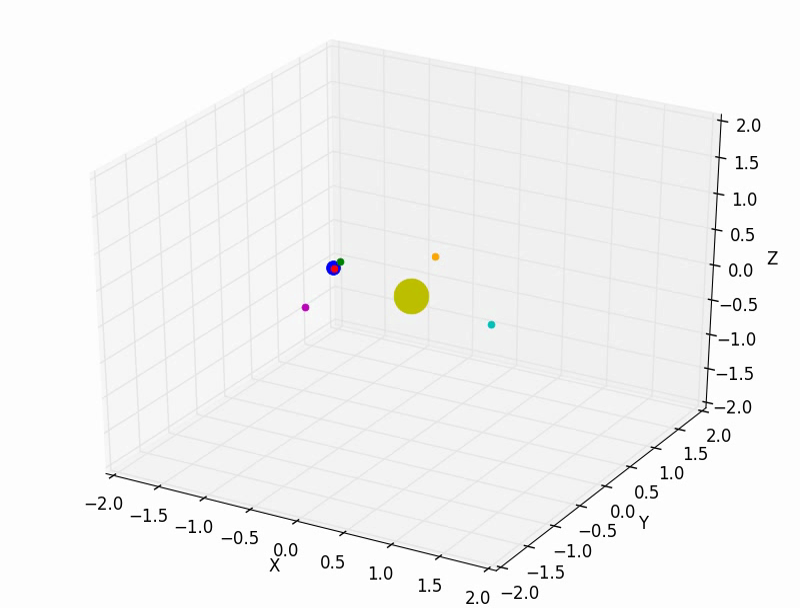
\includegraphics[width=\linewidth]{figures/lagrange_points/lagrange_points_l2_vx_001_1.png}
  \subcaption{}\label{fig:lagrange_points_l2_vx_001_fig1}
\endminipage\hfill
\minipage{0.5\textwidth}
  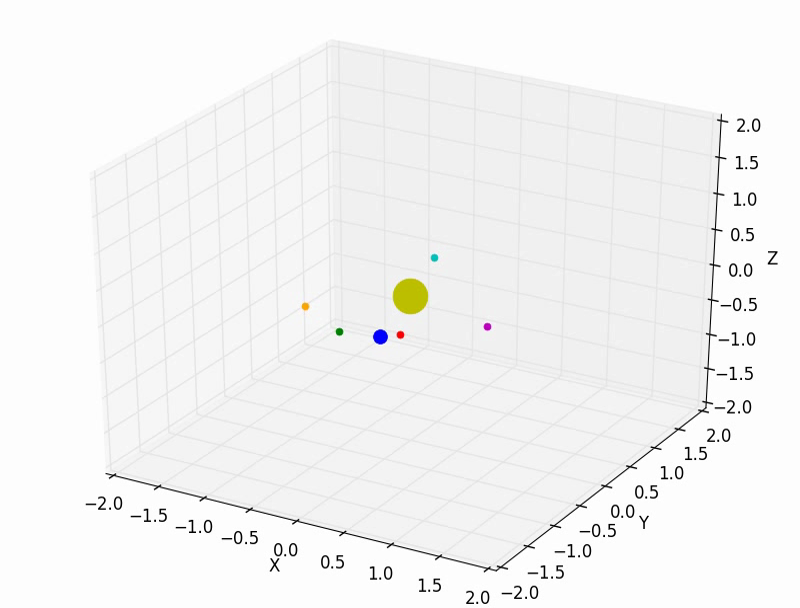
\includegraphics[width=\linewidth]{figures/lagrange_points/lagrange_points_l2_vx_001_2.png}
  \subcaption{}\label{fig:lagrange_points_l2_vx_001_fig2}
\endminipage\hfill
\minipage{0.5\textwidth}%
  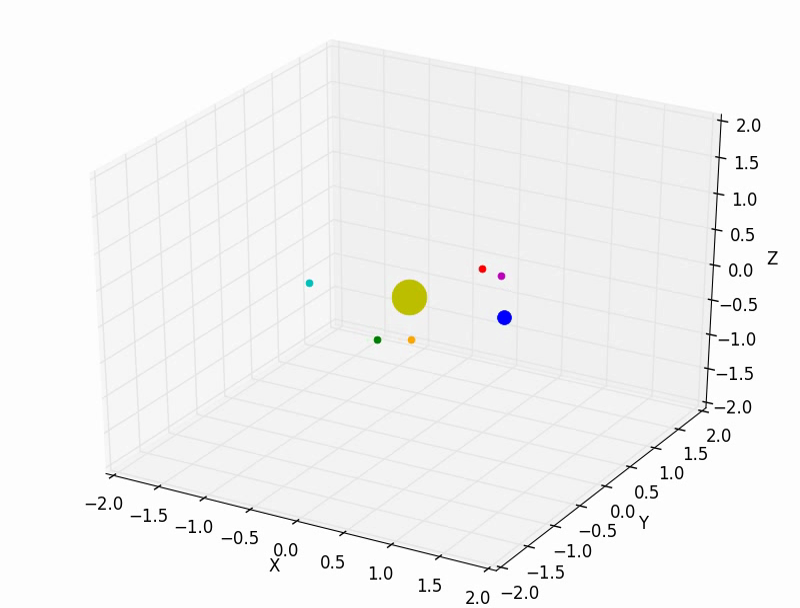
\includegraphics[width=\linewidth]{figures/lagrange_points/lagrange_points_l2_vx_001_3.png}
  \subcaption{}\label{fig:lagrange_points_l2_vx_001_fig3}
\endminipage
\minipage{0.5\textwidth}%
  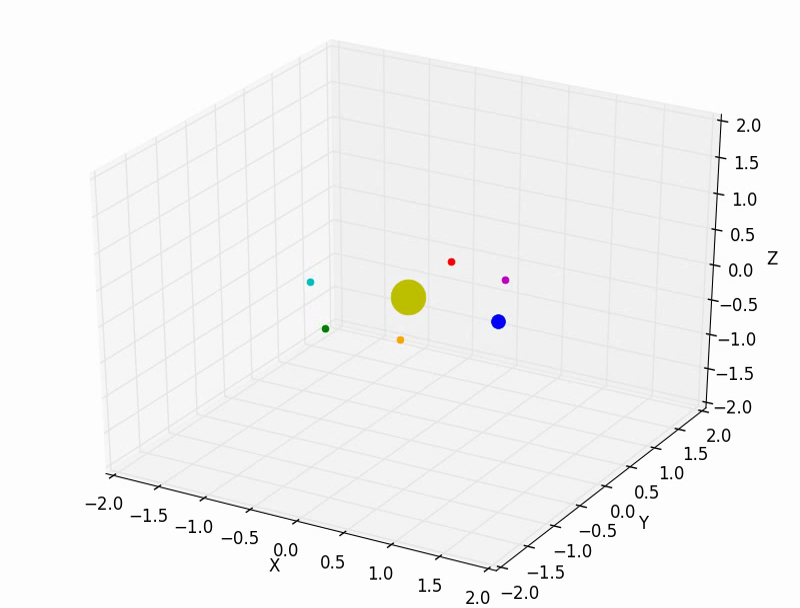
\includegraphics[width=\linewidth]{figures/lagrange_points/lagrange_points_l2_vx_001_4.png}
  \subcaption{}\label{fig:lagrange_points_l2_vx_001_fig4}
\endminipage
\caption{Orbits of the five Lagrange points of Sun-Earth system plotted over a time period of five years, $x$ component of L2 velocity has been perturbed by 1$\%$ angular velocity of Earth.
(\ref{fig:lagrange_points_l2_vx_001_fig1}) Initial orbit drift. 
(\ref{fig:lagrange_points_l2_vx_001_fig2}) Continued orbit drift. 
(\ref{fig:lagrange_points_l2_vx_001_fig3}) Continued orbit drift. 
(\ref{fig:lagrange_points_l2_vx_001_fig4}) End positions.}\label{fig:lagrange_points_l2_vx_001}
\end{figure}

We can see in these sets of plots that the orbit of the L2 point, which we already noted to be unstable, begins drifting much earlier in its orbit under this perturbation (figure \ref{fig:lagrange_points_l2_vx_001_fig1}). If we compare the positions of the L2 point in figure \ref{fig:lagrange_points_l2_vx_001} with its positions in figure \ref{fig:lagrange_points_stability} we can see that it does follow the same basic orbit, however its positions continues to drift at a much higher rate, thus increasing its instability. Now looking at figure \ref{fig:lagrange_points_l4_vx_001} we can see how L4 evolves after a 1$\%$ boost to the $x$ component of its velocity.\\
\pagebreak
\begin{figure}[!htb]
\minipage{0.5\textwidth}
  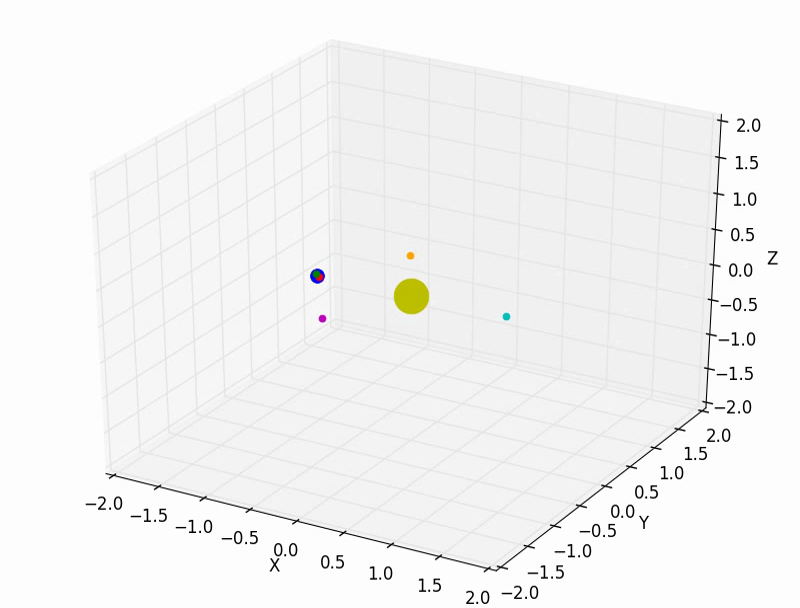
\includegraphics[width=\linewidth]{figures/lagrange_points/lagrange_points_l4_vx_001_1.png}
  \subcaption{}\label{fig:lagrange_points_l4_vx_001_fig1}
\endminipage\hfill
\minipage{0.5\textwidth}
  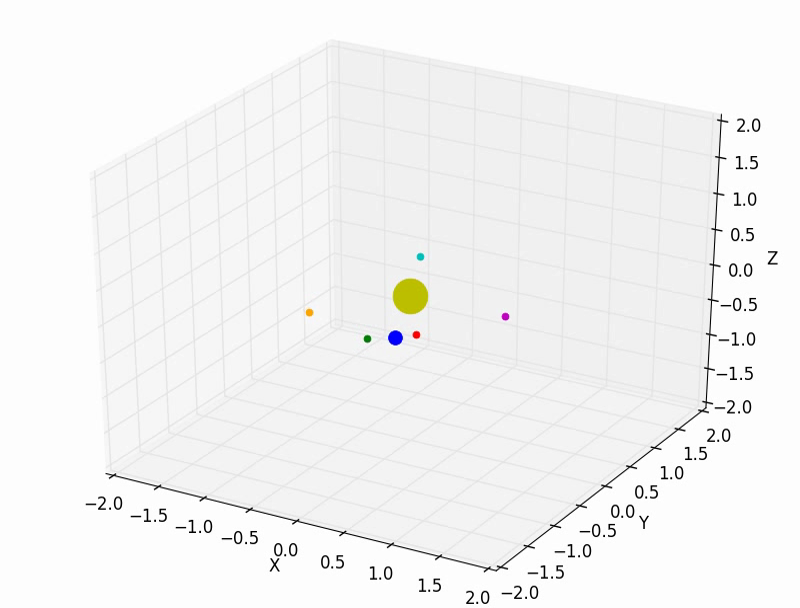
\includegraphics[width=\linewidth]{figures/lagrange_points/lagrange_points_l4_vx_001_2.png}
  \subcaption{}\label{fig:lagrange_points_l4_vx_001_fig2}
\endminipage\hfill
\minipage{0.5\textwidth}%
  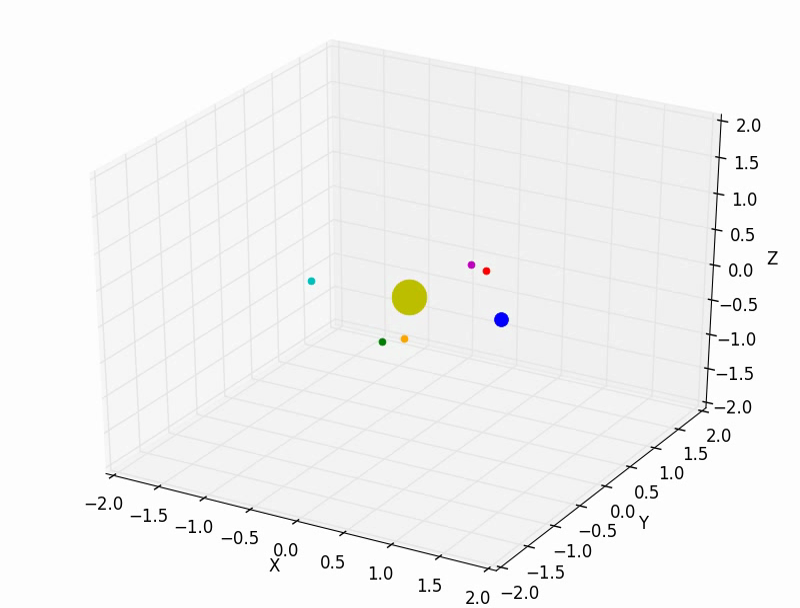
\includegraphics[width=\linewidth]{figures/lagrange_points/lagrange_points_l4_vx_001_3.png}
  \subcaption{}\label{fig:lagrange_points_l4_vx_001_fig3}
\endminipage
\minipage{0.5\textwidth}%
  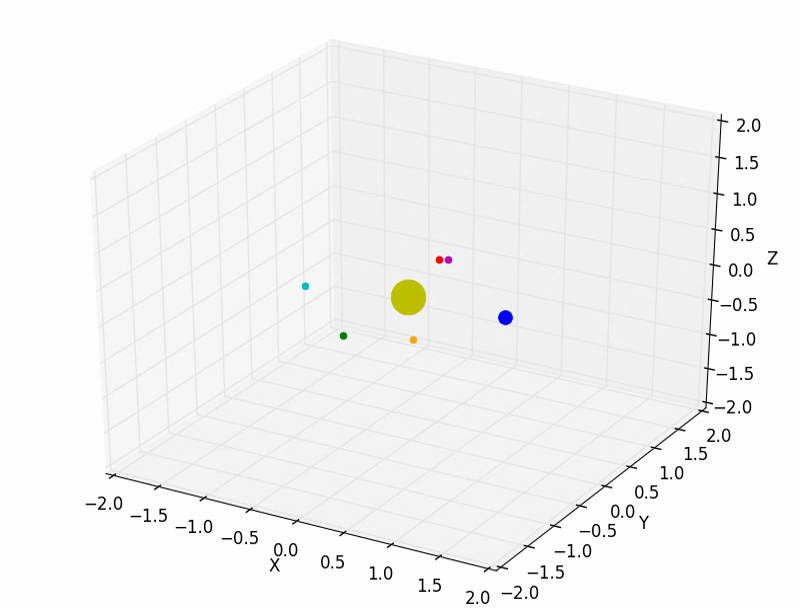
\includegraphics[width=\linewidth]{figures/lagrange_points/lagrange_points_l4_vx_001_4.png}
  \subcaption{}\label{fig:lagrange_points_l4_vx_001_fig4}
\endminipage
\caption{Orbits of the five Lagrange points of Sun-Earth system plotted over a time period of five years, $x$ component of L4 velocity has been perturbed by 1$\%$ angular velocity of Earth.
(\ref{fig:lagrange_points_l4_vx_001_fig1}) Initial orbit drift. 
(\ref{fig:lagrange_points_l4_vx_001_fig2}) Continued orbit drift. 
(\ref{fig:lagrange_points_l4_vx_001_fig3}) Continued orbit drift. 
(\ref{fig:lagrange_points_l4_vx_001_fig4}) End positions.}\label{fig:lagrange_points_l4_vx_001}
\end{figure}

We can see here that that L4 point remains relatively stable throughout its orbit, however it is still perturbed slightly in figure \ref{fig:lagrange_points_l4_vx_001_fig2} and even more so by figure \ref{fig:lagrange_points_l4_vx_001_fig3}. Comparing figure \ref{fig:lagrange_points_l4_vx_001_fig4} with figure \ref{fig:lagrange_points_stability_fig4} we can see just how far this perturbation has caused the L4 point to drift from its unperturbed final position. The same method was carried out for the $y$ components of the velocity with similar effects for both the L2 (figure \ref{fig:lagrange_points_l2_vy_001}) and L4 points (figure \ref{fig:lagrange_points_l4_vy_001}). Plots of these instances can be found within A.1. From the results of these plots we can see that a small perturbation of 1$\%$ of the angular velocity of the Earth to either the $x$ or $y$ components of velocity is enough to shift both the L2 and L4 Lagrange points from their initial orbits by a small amount. This amount of perturbation is not enough to completely disrupt their orbits however.\\

A far more dramatic disruption of the orbits can be seen when the velocities are perturbed by $10\%$. Plots of these instances can also be found within A.1. This level of perturbation is enough to severely disrupt the orbits of objects located in these points.
   
\pagebreak
\subsection{3-Body Scattering}

The goal of this section was to simulate a binary system of stars, then watch the effects of a third star entering and interacting with the existing binary system. The algorithm used the same concept as the prior two, where initial conditions where given, and the rest of the phase space coordinates were integrated using RK4. The second order differential equations needed to be solved were as follows:
\begin{align}
\frac{d\ddot{\vec{r}_1}}{dt} &= -Gm_2 \frac{\vec{r}_1-\vec{r}_2}{\left| \vec{r}_1- \vec{r}_2\right|^3} - Gm_3 \frac{\vec{r}_1-\vec{r}_3}{\left| \vec{r}_1- \vec{r}_3\right|^3} \\
\frac{d\ddot{\vec{r}_2}}{dt} &= -Gm_1 \frac{\vec{r}_2-\vec{r}_1}{\left| \vec{r}_2- \vec{r}_1\right|^3} - Gm_3 \frac{\vec{r}_2-\vec{r}_3}{\left| \vec{r}_2- \vec{r}_3\right|^3} \\
\frac{d\ddot{\vec{r}_3}}{dt} &= -Gm_1 \frac{\vec{r}_3-\vec{r}_1}{\left| \vec{r}_3- \vec{r}_1\right|^3} - Gm_2 \frac{\vec{r}_3-\vec{r}_2}{\left| \vec{r}_3- \vec{r}_2\right|^3}
\end{align}
6 different cases with different initial conditions will be shown and discussed in the following section. The images of the simulations can be found in the appendix and each animation can be found inside the 'animations' folder.
\subsubsection{Testing the Binary system}
Before we begun simulating a 3 body scatter, a functioning binary star system must first be tested to confirm that energy conservation and that the algorithm worked as intended. The two binary stars had the following characteristics:
\begin{table}[!htb]
\centering
\begin{tabular}{| c | c | c | c |}
\hline
Star & Mass ($M_{\odot}$) & Radius ($R_{\odot}$ ) & Initial Coordinates (x,y,z) \\
\hline
1 & 1 & 1 & (5$R_{\odot}$,0,0) \\
\hline
2 & 1 & 1 & ($-$5$R_{\odot}$,0,0) \\
\hline
\multicolumn{4}{|c|}{Duration of simulation: 11 days} \\
\hline
\end{tabular}
\end{table}
 Running the code with these given parameters generated the animation 'Binary\_Test\_Case.mp4' file. The two stars did indeed orbited about their center of mass (the origin) and did not deviate from the center. It was also noted that their separation remained constant which confirmed energy conservation. Their initial velocities were calculated from Newton's second law in the following manner:
\begin{align}
\frac{v_1^2}{d_1} &= G \frac{m_2}{\left( d_1 + d_2 \right)^2} \\
\frac{v_2^2}{d_2} &= G \frac{m_1}{\left( d_1 + d_2 \right)^2} 
\end{align}
Where $v_1$,$v_2$ were the initial velocities, $m_1$,$m_2$ were the respective masses, and $d_1$,  $d_2$ were the distances from the center of the mass of the binary system.\\[2ex]
Now that the binary system was confirmed to be functioning properly, the third star was then added to the system.
\subsubsection{Outer Orbit of the Third Star}
If the third star had an appropriate initial velocity for a stable orbit corresponding to it's initial position, it should in theory be possible to have the third star orbit the binary system in the center as if the binary system was a point mass in the center. The stars in the following animation 'Third\_Orbit.mp4' had the following characteristics:
\begin{table}[!htb]
\centering
\begin{tabular}{| c | c | c | c |}
\hline
Star & Mass ($M_{\odot}$) & Radius ($R_{\odot}$ ) & Initial Coordinates (x,y,z)\\
\hline
1 & 15 & 1 & (5$R_{\odot}$,0,0) \\
\hline
2 & 15 & 1 & ($-$5$R_{\odot}$,0,0) \\
\hline 
3 & 3 & 1 & (0,-50$R_{\odot}$,0) \\
\hline
\multicolumn{4}{|c|}{Duration of simulation: 36.5 days} \\
\hline
\end{tabular}
\end{table}
As the third star orbited the binary system, the center of mass of the binary system drifted towards the initial position of the third star, after several orbits, the system of stars disappear from the screen. To find initial velocity the third star needed to obtain a stable orbit, the following equation was implemented:
\begin{align}
v_i = \sqrt{G\frac{m_1 + m_2}{d_3}}
\end{align}
Where $d_3$ is the distance from the third star to the center of mass of the binary system.
\subsubsection{Gravity Assist}
When the third star whose mass was much smaller in comparison to the binary system masses approached the system from the side with velocity greater than the stable orbit velocity, it exhibited an effect similar to gravity assist. The binary system sling-shotted the third star and caused it's trajectory to change. The stars in the following animation 'gravity\_assist.mp4' had the following characteristics:
\begin{table}[!htb]
\centering
\begin{tabular}{| c | c | c | c |}
\hline
Star & Mass ($M_{\odot}$) & Radius ($R_{\odot}$ ) & Initial Coordinates (x,y,z)\\
\hline
1 & 50 & 1 & (5$R_{\odot}$,0,0) \\
\hline
2 & 50 & 1 & ($-$5$R_{\odot}$,0,0) \\
\hline 
3 & 1 & 1 & (60$R_{\odot}$,60$R_{\odot}$,0) \\
\hline
\multicolumn{4}{|c|}{Duration of simulation: 5.5 days} \\
\hline
\end{tabular}
\end{table}
When the speed of an approaching object was too higher than the stable orbit velocity, a slingshot effect was seen in the simulation (hyperbolic orbit), where the binary system attempts to pull the third star into the system, however the third star escapes it's pull as it's velocity was too high. The binary system merely changes the trajectory of the third star as it passes by.
\subsubsection{3 Body Scatter}
To scatter the binary system, we placed the third star in a direct trajectory with the center of mass of the binary system. In this specific simulation, 'ThreeBody2\_scatter.mp4', the third star had an initial velocity of 0 and all stars had the following characteristics:
\begin{table}[!htb]
\centering
\begin{tabular}{| c | c | c | c |}
\hline
Star & Mass ($M_{\odot}$) & Radius ($R_{\odot}$ ) & Initial Coordinates (x,y,z)\\
\hline
1 & 4 & 1 & (5$R_{\odot}$,0,0) \\
\hline
2 & 4 & 1 & ($-$5$R_{\odot}$,0,0) \\
\hline 
3 & 5 & 1 & (0,45$R_{\odot}$,0) \\
\hline
\multicolumn{4}{|c|}{Duration of simulation: 5.5 days} \\
\hline
\end{tabular}
\end{table}
As the third star begun with 0 initial velocity, it took a while before the star interacted with the binary system. As the third star came in contact with one of the stars, an unphysical event happened, where the third star collided with the the other star, causing a launch of the two stars as their centers came too close. The acceleration dramatically increased as their separation distance was approaching zero. This caused a scattering behaviour and the bounded gravitational energy completely converted to kinetic energy.
\subsubsection{Unphysical Behaviours}
When we ran this simulation numerous times, changing the initial conditions each time, we ran into many cases where a star seemed to collide into another one, this usually created an unphysical effect where the stars spun at high speeds around each other and launched in opposite directions. This was shown in the the animation 'ThreeBody3\_initvel.mp4', where the stars had the following characteristics:
\begin{table}[!htb]
\centering
\begin{tabular}{| c | c | c | c |}
\hline
Star & Mass ($M_{\odot}$) & Radius ($R_{\odot}$ ) & Initial Coordinates (x,y,z)\\
\hline
1 & 10 & 1 & (5$R_{\odot}$,0,0) \\
\hline
2 & 10 & 1 & ($-$5$R_{\odot}$,0,0) \\
\hline 
3 & 10 & 1 & (0,45$R_{\odot}$,0) \\
\hline
\multicolumn{4}{|c|}{Duration of simulation: 11 days} \\
\hline
\end{tabular}
\end{table}
This simulation showed the flaw in a this type of simulation. Slight initial condition changes could severely alter the end result of the simulation. The biggest flaw in our algorithm was that each star was treated like a point mass. This caused stars to "go inside" of each other instead of a collision. In numerous different cases during testing, such "collisions" happened and stars are launched at astonishing high speeds from one another. 
\subsubsection{Stolen Star}
After tweaking some changes, we decided to make the approaching star more massive than the binary stars and observe any interesting changes. The third star stole one of the stars as it interacted with the system and a smaller binary system was made between the third star and one of the binary stars. The stars in the animation 'ThreeBody4\_StolenStar.mp4' had the following characteristics:
\begin{table}[!htb]
\centering
\begin{tabular}{| c | c | c | c |}
\hline
Star & Mass ($M_{\odot}$) & Radius ($R_{\odot}$ ) & Initial Coordinates (x,y,z)\\
\hline
1 & 4 & 1 & (5$R_{\odot}$,0,0) \\
\hline
2 & 4 & 1 & ($-$5$R_{\odot}$,0,0) \\
\hline 
3 & 6 & 1 & (0,45$R_{\odot}$,0) \\
\hline
\multicolumn{4}{|c|}{Duration of simulation: 18.25 days} \\
\hline
\end{tabular}
\end{table}
This case was interesting as it shows how a bigger mass can affect a smaller binary system. The binary system accelerated towards the third star and vise versa, the binary system collapsed and started to quickly spin around the third star. One of the binary stars had enough velocity to escape the third star, however, the other binary star was now bound to the third star, where another binary system began. This new binary system consisted of a bigger mass and a smaller mass, so consequently, the center of mass was closer to the bigger mass and the smaller mass made elliptical orbits around the third star.

\pagebreak
\section{Discussion}

Using RK4 for our simulations conserves energy and gives the closest results to the exact solutions for our test cases. Unfortunately, there are limitations to using this. For instance, RK4 is the most computationally expensive of the other methods, as it carries out more floating point operations in a single step. This is the price we have to pay for accuracy, as the other methods while computationally less expensive are less accurate and conserve energy more poorly. An adaptive RK4 method could instead be used to reduce resources and computation time, as it would use less time steps to calculate the next positions of the objects further away from the origin, reducing the number of operations performed.\\

There are also limitations to our time step choices. To save on memory and computational time while also showing as much as possible of the galaxy collision simulations, a choice of time steps of 3 million years out to 5 billion years was chosen. Having such massive time steps results in some of the stars near the center of the two galaxies flying out and escaping the system as the time steps are too large for the numerical method to accurately calculate these stars' next positions. What happens is that these stars have high enough orbital velocities that the RK4 method calculates their next position in 3 million years as being further away radially from their true position, far enough such that their velocities are greater than the escape velocity of the star at that radial position. As such, at the beginning of each galaxy collision simulation, many stars can appear to shoot out from the centre of both galaxies, resulting in holes near the centre of the galaxies where there are no stars. An obvious solution to this is to use smaller time steps, although at the cost of computation time and memory. Another solution is to use a minimum radius such that no stars are placed within so that no stars shoot out from the centre of each galaxy.\\

The choice of appropriate time steps is also very important in studying the orbits of objects within the Lagrange points. As the majority of these orbits are only semi stable (L1, L2 and L3) small inconsistencies due to having too large of times steps can have large impacts on the evolution of orbital trajectories. With the L1 and L2 Lagrange points being so close to the Earth there were many problems with determining the correct time steps to allow the instability of these orbits to arise. Many simulations were run in which the objects orbiting in these points were trapped within the Earth's orbit. As always the choice to simply use smaller time steps to avoid this problem is always available, however this is at the cost of computation time which is always an important resource.\\

The time steps in the 3 body scatter simulation were made to be very small (5 minutes) as only 3 objects were being calculated for each time step. This ensured that energy was conserved as much as possible since the velocities were updated very frequently. However, the biggest concern from this simulation was the stars being point masses. Since there's no designated radius of a star in the algorithm, a star could approach another star without colliding. This caused unphysical cases where two stars that have "collided" launched at very high speeds away from each other due to acceleration due to gravity increasing dramatically as their separation decreases to 0. During our time of running the simulation, more often than not, this situation of collision would occur. However, this should be expected as stars with low enough velocities will succumb to gravity's pull and collide with each other.\\

\pagebreak
\section{Conclusions}

The goal of this project was to develop an integration system to simulate a gravitational $N$-body system. Several methods of solving ODEs were tested in terms of their ability to conserve energy ad reproduce expected results. In the end a 4$^{th}$ order Runge-Kutta method was chosen as it was shown to conserve energy, reliably reproduce results and best suited the needs of this project.\\

The collision of two galaxies with as many as 10 000 particles was successfully simulated. It was found that the collisions were heavily dependent on the orbital angular momentum and the angular momentum of the collision. When these two values were aligned the results were such that the incoming galaxy encountered a much higher level of disruption to the stars in it's orbit.\\

The orbits associated with the Lagrange points of the Sun-Earth system were studied. It was found that the L1, L2 and L3 points were all unstable over time while the L4 and L5 points are stable orbits. It was also found that changing the $x$ or $y$ velocity at these points by as little as 1$\%$ of the angular velocity of the Earth is enough to shift object in these orbits. It takes a shift of as much as 10$\%$ of the angular velocity of the Earth to completely disrupt these orbits.\\

In the 3 body scatter experiment, numerous simulations with different initial conditions were ran to observe the behaviour of the stars. The results highly varied depending on the initial conditions set, a small change in initial conditions led to a big change in the end. To further increase the accuracy of this algorithm, stars should not have been treated as point masses but as a distribution of mass with a designated radius instead. Also, during a collision, the algorithm should attach the two stars as one (to simulate stellar collision) instead of launching them away from each other.\\

\pagebreak
\appendix

\section{Appendices}

\subsection{Lagrange Points: Additional Figures}

\begin{figure}[!htb]
\minipage{0.25\textwidth}
  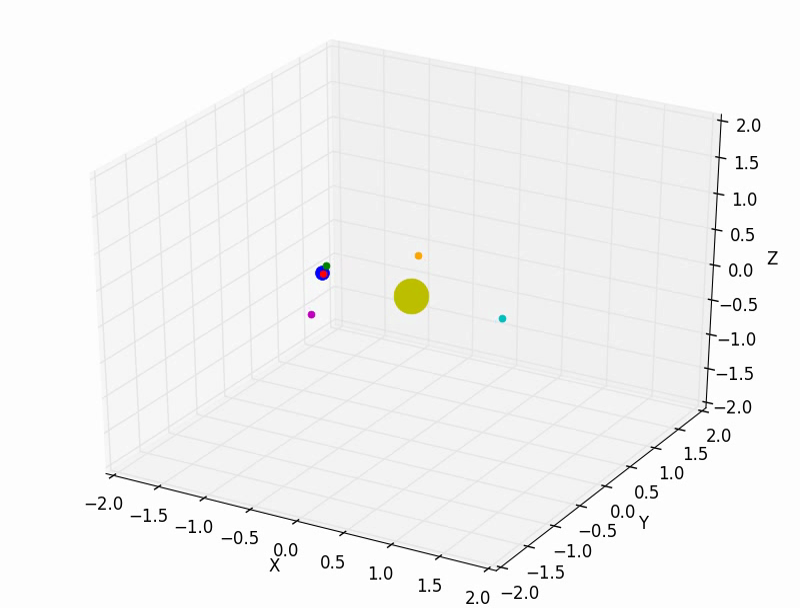
\includegraphics[width=\linewidth]{figures/lagrange_points/lagrange_points_l2_vy_001_1.png}
  \subcaption{}\label{fig:lagrange_points_l2_vy_001_fig1}
\endminipage\hfill
\minipage{0.25\textwidth}
  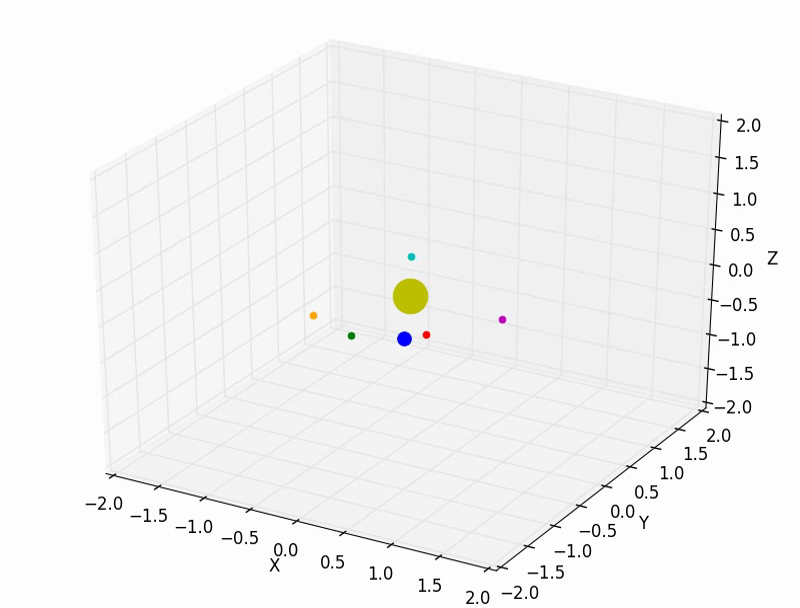
\includegraphics[width=\linewidth]{figures/lagrange_points/lagrange_points_l2_vy_001_2.png}
  \subcaption{}\label{fig:lagrange_points_l2_vy_001_fig2}
\endminipage\hfill
\minipage{0.25\textwidth}%
  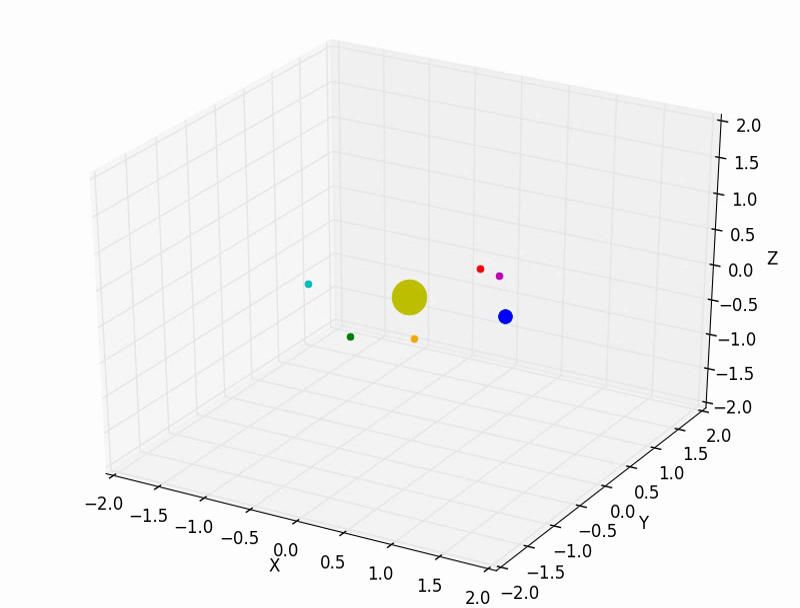
\includegraphics[width=\linewidth]{figures/lagrange_points/lagrange_points_l2_vy_001_3.png}
  \subcaption{}\label{fig:lagrange_points_l2_vy_001_fig3}
\endminipage
\minipage{0.25\textwidth}%
  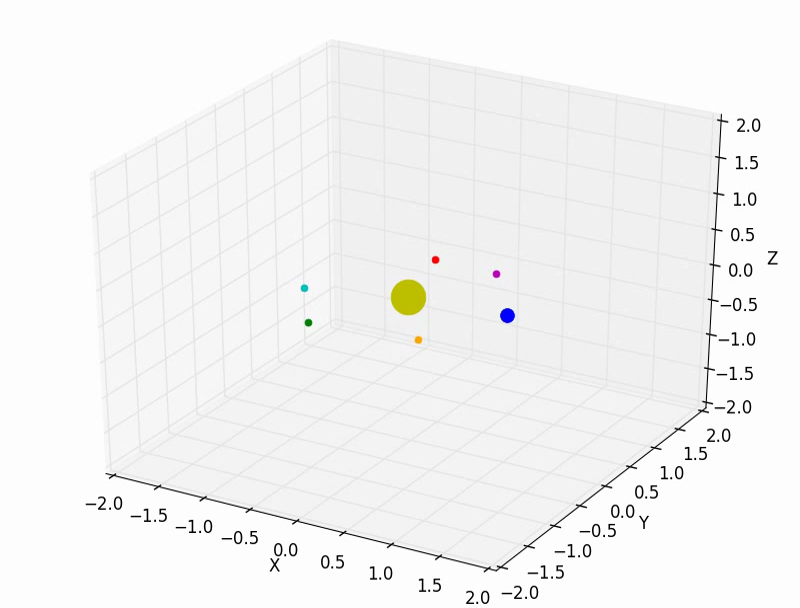
\includegraphics[width=\linewidth]{figures/lagrange_points/lagrange_points_l2_vy_001_4.png}
  \subcaption{}\label{fig:lagrange_points_l2_vy_001_fig4}
\endminipage
\caption{Orbits of the five Lagrange points of Sun-Earth system plotted over a time period of five years, $y$ component of L2 velocity has been perturbed by 1$\%$ angular velocity of Earth.
(\ref{fig:lagrange_points_l2_vy_001_fig1}) 
(\ref{fig:lagrange_points_l2_vy_001_fig2}) 
(\ref{fig:lagrange_points_l2_vy_001_fig3}) 
(\ref{fig:lagrange_points_l2_vy_001_fig4})}\label{fig:lagrange_points_l2_vy_001}
\end{figure}

\begin{figure}[!htb]
\minipage{0.25\textwidth}
  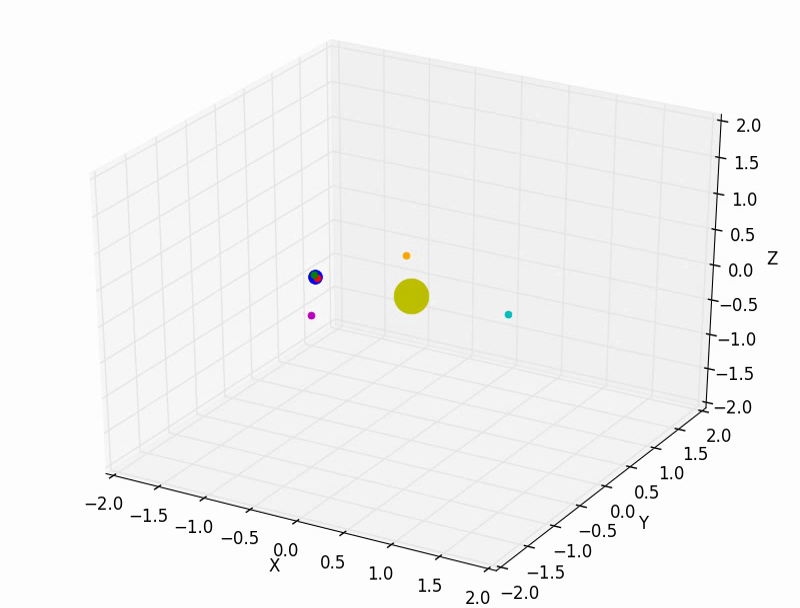
\includegraphics[width=\linewidth]{figures/lagrange_points/lagrange_points_l4_vy_001_1.png}
  \subcaption{}\label{fig:lagrange_points_l4_vy_001_fig1}
\endminipage\hfill
\minipage{0.25\textwidth}
  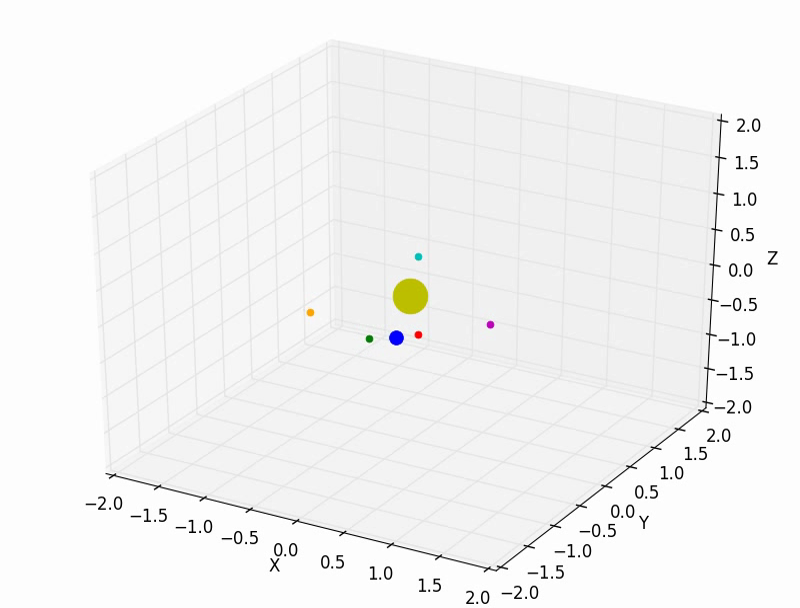
\includegraphics[width=\linewidth]{figures/lagrange_points/lagrange_points_l4_vy_001_2.png}
  \subcaption{}\label{fig:lagrange_points_l4_vy_001_fig2}
\endminipage\hfill
\minipage{0.25\textwidth}%
  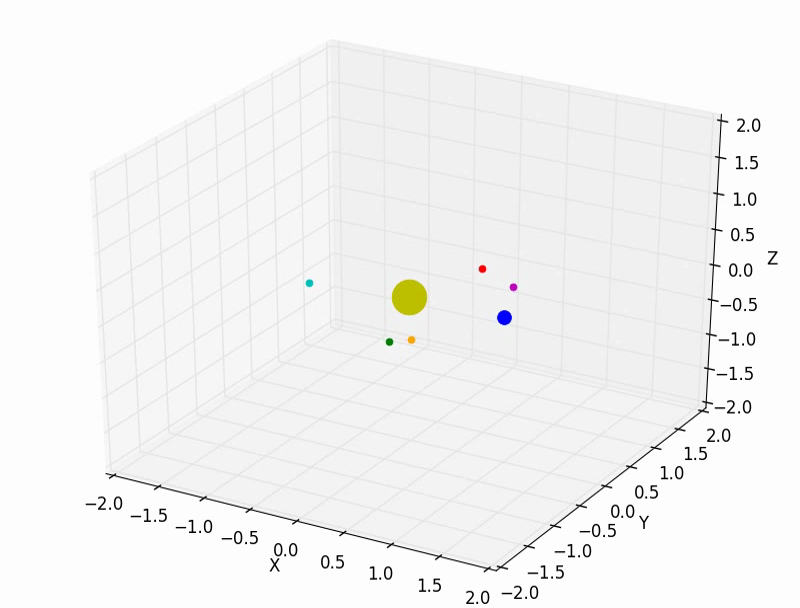
\includegraphics[width=\linewidth]{figures/lagrange_points/lagrange_points_l4_vy_001_3.png}
  \subcaption{}\label{fig:lagrange_points_l4_vy_001_fig3}
\endminipage
\minipage{0.25\textwidth}%
  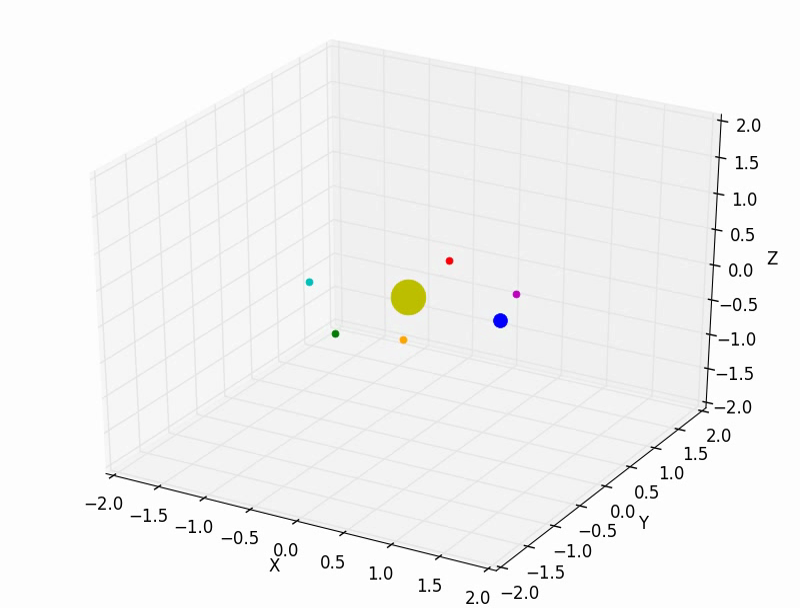
\includegraphics[width=\linewidth]{figures/lagrange_points/lagrange_points_l4_vy_001_4.png}
  \subcaption{}\label{fig:lagrange_points_l4_vy_001_fig4}
\endminipage
\caption{Orbits of the five Lagrange points of Sun-Earth system plotted over a time period of five years, $y$ component of L4 velocity has been perturbed by 1$\%$ angular velocity of Earth.
(\ref{fig:lagrange_points_l4_vy_001_fig1}) 
(\ref{fig:lagrange_points_l4_vy_001_fig2}) 
(\ref{fig:lagrange_points_l4_vy_001_fig3}) 
(\ref{fig:lagrange_points_l4_vy_001_fig4})}\label{fig:lagrange_points_l4_vy_001}
\end{figure}

\begin{figure}[!htb]
\minipage{0.25\textwidth}
  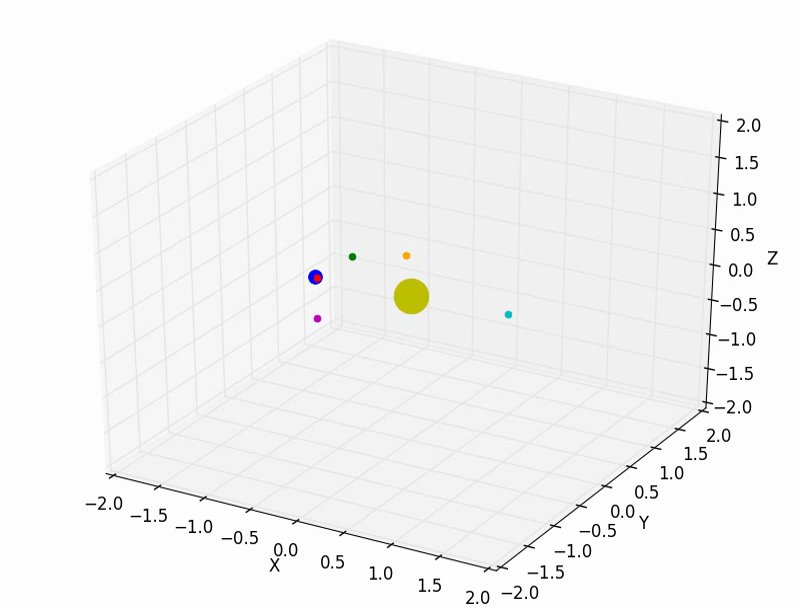
\includegraphics[width=\linewidth]{figures/lagrange_points/lagrange_points_l2_vx_01_1.png}
  \subcaption{}\label{fig:lagrange_points_l2_vx_01_fig1}
\endminipage\hfill
\minipage{0.25\textwidth}
  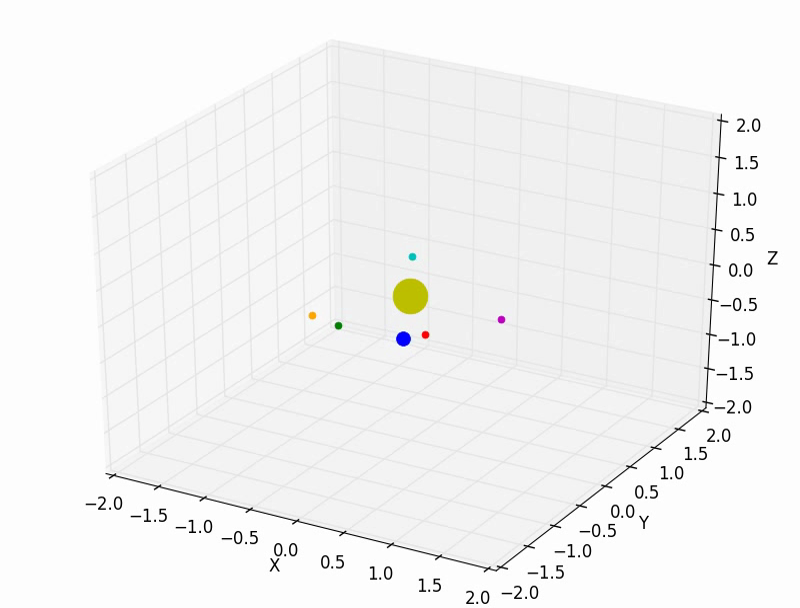
\includegraphics[width=\linewidth]{figures/lagrange_points/lagrange_points_l2_vx_01_2.png}
  \subcaption{}\label{fig:lagrange_points_l2_vx_01_fig2}
\endminipage\hfill
\minipage{0.25\textwidth}%
  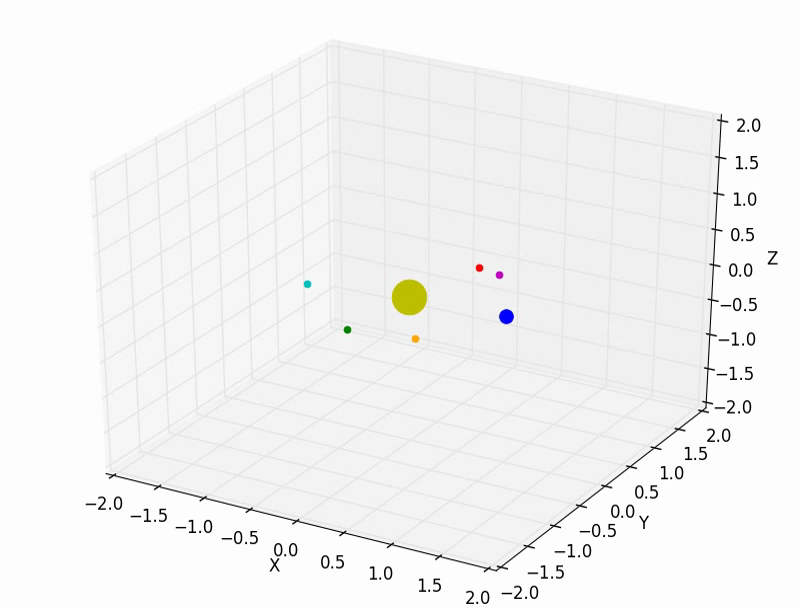
\includegraphics[width=\linewidth]{figures/lagrange_points/lagrange_points_l2_vx_01_3.png}
  \subcaption{}\label{fig:lagrange_points_l2_vx_01_fig3}
\endminipage
\minipage{0.25\textwidth}%
  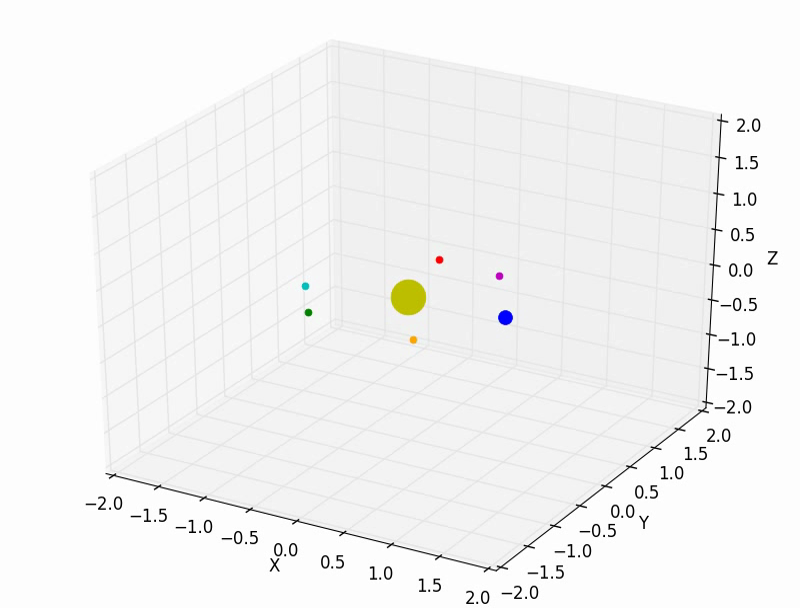
\includegraphics[width=\linewidth]{figures/lagrange_points/lagrange_points_l2_vx_01_4.png}
  \subcaption{}\label{fig:lagrange_points_l2_vx_01_fig4}
\endminipage
\caption{Orbits of the five Lagrange points of Sun-Earth system plotted over a time period of five years, $x$ component of L2 velocity has been perturbed by 10$\%$ angular velocity of Earth.
(\ref{fig:lagrange_points_l2_vx_01_fig1}) 
(\ref{fig:lagrange_points_l2_vx_01_fig2}) 
(\ref{fig:lagrange_points_l2_vx_01_fig3}) 
(\ref{fig:lagrange_points_l2_vx_01_fig4})}\label{fig:lagrange_points_l2_vx_01}
\end{figure}

\begin{figure}[!htb]
\minipage{0.25\textwidth}
  \includegraphics[width=\linewidth]{figures/lagrange_points/lagrange_points_l2_vy_01_1.png}
  \subcaption{}\label{fig:lagrange_points_l2_vy_01_fig1}
\endminipage\hfill
\minipage{0.25\textwidth}
  \includegraphics[width=\linewidth]{figures/lagrange_points/lagrange_points_l2_vy_01_2.png}
  \subcaption{}\label{fig:lagrange_points_l2_vy_01_fig2}
\endminipage\hfill
\minipage{0.25\textwidth}%
  \includegraphics[width=\linewidth]{figures/lagrange_points/lagrange_points_l2_vy_01_3.png}
  \subcaption{}\label{fig:lagrange_points_l2_vy_01_fig3}
\endminipage
\minipage{0.25\textwidth}%
  \includegraphics[width=\linewidth]{figures/lagrange_points/lagrange_points_l2_vy_01_4.png}
  \subcaption{}\label{fig:lagrange_points_l2_vy_01_fig4}
\endminipage
\caption{Orbits of the five Lagrange points of Sun-Earth system plotted over a time period of five years, $y$ component of L2 velocity has been perturbed by 10$\%$ angular velocity of Earth.
(\ref{fig:lagrange_points_l2_vy_01_fig1}) 
(\ref{fig:lagrange_points_l2_vy_01_fig2}) 
(\ref{fig:lagrange_points_l2_vy_01_fig3}) 
(\ref{fig:lagrange_points_l2_vy_01_fig4})}\label{fig:lagrange_points_l2_vy_01}
\end{figure}

\begin{figure}[!htb]
\minipage{0.25\textwidth}
  \includegraphics[width=\linewidth]{figures/lagrange_points/lagrange_points_l4_vx_01_1.png}
  \subcaption{}\label{fig:lagrange_points_l4_vx_01_fig1}
\endminipage\hfill
\minipage{0.25\textwidth}
  \includegraphics[width=\linewidth]{figures/lagrange_points/lagrange_points_l4_vx_01_2.png}
  \subcaption{}\label{fig:lagrange_points_l4_vx_01_fig2}
\endminipage\hfill
\minipage{0.25\textwidth}%
  \includegraphics[width=\linewidth]{figures/lagrange_points/lagrange_points_l4_vx_01_3.png}
  \subcaption{}\label{fig:lagrange_points_l4_vx_01_fig3}
\endminipage
\minipage{0.25\textwidth}%
  \includegraphics[width=\linewidth]{figures/lagrange_points/lagrange_points_l4_vx_01_4.png}
  \subcaption{}\label{fig:lagrange_points_l4_vx_01_fig4}
\endminipage
\caption{Orbits of the five Lagrange points of Sun-Earth system plotted over a time period of five years, $x$ component of L4 velocity has been perturbed by 10$\%$ angular velocity of Earth.
(\ref{fig:lagrange_points_l4_vx_01_fig1}) 
(\ref{fig:lagrange_points_l4_vx_01_fig2}) 
(\ref{fig:lagrange_points_l4_vx_01_fig3}) 
(\ref{fig:lagrange_points_l4_vx_01_fig4})}\label{fig:lagrange_points_l4_vx_01}
\end{figure}

\begin{figure}[!htb]
\minipage{0.25\textwidth}
  \includegraphics[width=\linewidth]{figures/lagrange_points/lagrange_points_l4_vy_01_1.png}
  \subcaption{}\label{fig:lagrange_points_l4_vy_01_fig1}
\endminipage\hfill
\minipage{0.25\textwidth}
  \includegraphics[width=\linewidth]{figures/lagrange_points/lagrange_points_l4_vy_01_2.png}
  \subcaption{}\label{fig:lagrange_points_l4_vy_01_fig2}
\endminipage\hfill
\minipage{0.25\textwidth}%
  \includegraphics[width=\linewidth]{figures/lagrange_points/lagrange_points_l4_vy_01_3.png}
  \subcaption{}\label{fig:lagrange_points_l4_vy_01_fig3}
\endminipage
\minipage{0.25\textwidth}%
  \includegraphics[width=\linewidth]{figures/lagrange_points/lagrange_points_l4_vy_01_4.png}
  \subcaption{}\label{fig:lagrange_points_l4_vy_01_fig4}
\endminipage
\caption{Orbits of the five Lagrange points of Sun-Earth system plotted over a time period of five years, $y$ component of L4 velocity has been perturbed by 10$\%$ angular velocity of Earth.
(\ref{fig:lagrange_points_l4_vy_01_fig1}) 
(\ref{fig:lagrange_points_l4_vy_01_fig2}) 
(\ref{fig:lagrange_points_l4_vy_01_fig3}) 
(\ref{fig:lagrange_points_l4_vy_01_fig4})}\label{fig:lagrange_points_l4_vy_01}
\end{figure}

\pagebreak
\subsection{3 Body Scattering: Additional Figures}

\begin{figure}[!htb]
\minipage{0.25\textwidth}
  \includegraphics[width=\linewidth]{figures/three_body/1_1.png}
  \subcaption{}\label{fig:1_1}
\endminipage\hfill
\minipage{0.25\textwidth}
  \includegraphics[width=\linewidth]{figures/three_body/1_2.png}
  \subcaption{}\label{fig:1_2}
\endminipage\hfill
\minipage{0.25\textwidth}
  \includegraphics[width=\linewidth]{figures/three_body/1_3.png}
  \subcaption{}\label{fig:1_3}
\endminipage
\minipage{0.25\textwidth}
  \includegraphics[width=\linewidth]{figures/three_body/1_4.png}
  \subcaption{}\label{fig:1_4}
\endminipage
\caption{ \textit{Testing the Binary system} - A test case to ensure that the binary system conserves energy and stays bound without any change in separation distance.
(\ref{fig:1_1}) 
(\ref{fig:1_2}) 
(\ref{fig:1_3}) 
(\ref{fig:1_4})}\label{fig:1}
\end{figure}

\begin{figure}[!htb]
\minipage{0.25\textwidth}
  \includegraphics[width=\linewidth]{figures/three_body/2_1.png}
  \subcaption{}\label{fig:2_1}
\endminipage\hfill
\minipage{0.25\textwidth}
  \includegraphics[width=\linewidth]{figures/three_body/2_2.png}
  \subcaption{}\label{fig:2_2}
\endminipage\hfill
\minipage{0.25\textwidth}
  \includegraphics[width=\linewidth]{figures/three_body/2_3.png}
  \subcaption{}\label{fig:2_3}
\endminipage
\minipage{0.25\textwidth}
  \includegraphics[width=\linewidth]{figures/three_body/2_4.png}
  \subcaption{}\label{fig:2_4}
\endminipage
\caption{ \textit{Outer Orbit of the Third Star} - Third star with a stable orbit around the binary system
(\ref{fig:2_1}) 
(\ref{fig:2_2}) 
(\ref{fig:2_3}) 
(\ref{fig:2_4})}\label{fig:2}
\end{figure}

\begin{figure}[!htb]
\minipage{0.25\textwidth}
  \includegraphics[width=\linewidth]{figures/three_body/3_1.png}
  \subcaption{}\label{fig:3_1}
\endminipage\hfill
\minipage{0.25\textwidth}
  \includegraphics[width=\linewidth]{figures/three_body/3_2.png}
  \subcaption{}\label{fig:3_2}
\endminipage\hfill
\minipage{0.25\textwidth}
  \includegraphics[width=\linewidth]{figures/three_body/3_3.png}
  \subcaption{}\label{fig:3_3}
\endminipage
\minipage{0.25\textwidth}
  \includegraphics[width=\linewidth]{figures/three_body/3_4.png}
  \subcaption{}\label{fig:3_4}
\endminipage
\caption{ \textit{Gravity Assist} - The approaching third star sling-shotted by the binary system
(\ref{fig:3_1}) 
(\ref{fig:3_2}) 
(\ref{fig:3_3}) 
(\ref{fig:3_4})}\label{fig:3}
\end{figure}

\begin{figure}[!htb]
\minipage{0.25\textwidth}
  \includegraphics[width=\linewidth]{figures/three_body/4_1.png}
  \subcaption{}\label{fig:4_1}
\endminipage\hfill
\minipage{0.25\textwidth}
  \includegraphics[width=\linewidth]{figures/three_body/4_2.png}
  \subcaption{}\label{fig:4_2}
\endminipage\hfill
\minipage{0.25\textwidth}
  \includegraphics[width=\linewidth]{figures/three_body/4_3.png}
  \subcaption{}\label{fig:4_3}
\endminipage
\minipage{0.25\textwidth}
  \includegraphics[width=\linewidth]{figures/three_body/4_4.png}
  \subcaption{}\label{fig:4_4}
\endminipage
\caption{ \textit{3 Body Scatter} - Incoming third star scatters the binary system and launches one of the binary stars away
(\ref{fig:4_1}) 
(\ref{fig:4_2}) 
(\ref{fig:4_3}) 
(\ref{fig:4_4})}\label{fig:4}
\end{figure}

\begin{figure}[!htb]
\minipage{0.25\textwidth}
  \includegraphics[width=\linewidth]{figures/three_body/5_1.png}
  \subcaption{}\label{fig:5_1}
\endminipage\hfill
\minipage{0.25\textwidth}
  \includegraphics[width=\linewidth]{figures/three_body/5_2.png}
  \subcaption{}\label{fig:5_2}
\endminipage\hfill
\minipage{0.25\textwidth}
  \includegraphics[width=\linewidth]{figures/three_body/5_3.png}
  \subcaption{}\label{fig:5_3}
\endminipage
\minipage{0.25\textwidth}
  \includegraphics[width=\linewidth]{figures/three_body/5_4.png}
  \subcaption{}\label{fig:5_4}
\endminipage
\caption{ \textit{Unphysical Behaviours} - Stars seemed to have collided and launched far away
(\ref{fig:5_1}) 
(\ref{fig:5_2}) 
(\ref{fig:5_3}) 
(\ref{fig:5_4})}\label{fig:5}
\end{figure}

\begin{figure}[!htb]
\minipage{0.25\textwidth}
  \includegraphics[width=\linewidth]{figures/three_body/6_1.png}
  \subcaption{}\label{fig:6_1}
\endminipage\hfill
\minipage{0.25\textwidth}
  \includegraphics[width=\linewidth]{figures/three_body/6_2.png}
  \subcaption{}\label{fig:6_2}
\endminipage\hfill
\minipage{0.25\textwidth}
  \includegraphics[width=\linewidth]{figures/three_body/6_3.png}
  \subcaption{}\label{fig:6_3}
\endminipage
\minipage{0.25\textwidth}
  \includegraphics[width=\linewidth]{figures/three_body/6_4.png}
  \subcaption{}\label{fig:6_4}
\endminipage
\caption{ \textit{Stolen Star} - Third star with high mass steals one of the binary stars and forms its own binary system
(\ref{fig:6_1}) 
(\ref{fig:6_2}) 
(\ref{fig:6_3}) 
(\ref{fig:6_4})}\label{fig:6}
\end{figure}

\end{document}